% -------------------------------------------------------------------------------------------------
%      MDSG Latex Framework
%      ============================================================================================
%      File:                  appendix.tex
%      Author(s):             Michael Duerr
%      Version:               1
%      Creation Date:         30. Mai 2010
%      Creation Date:         30. Mai 2010
%
%      Notes:                 - Place your appendix here
%                             - Use the same commands (`chapter', `section', ...) as in main text
% -------------------------------------------------------------------------------------------------
%
\chapter{Training Parameters}\label{ax:training_params}
\small{
    \begin{verbatim}
required arguments:
  --algo ALGO           Algorithm to use for training. Choose between 'ppo'
                        and 'dqn'.

optional arguments:
  -h, --help            show this help message and exit
  --seed SEED           Generate the same set of pseudo random constellations,
                        colors, positions, etc. every time the algorithm is
                        executed. (default: 1)
  --agents AGENTS       Amount of agents. (default: 2)
  --model MODEL         Path of the model inside the storage folder, if none
                        is given then a random name is generated. (default:
                        None)
  --capture CAPTURE     Boolean to enable capturing of the environment. The
                        outcome are in form of gifs. (default: True)
  --env ENV             Environment ID, choose between Empty-Grid-v0 for an
                        empty environment and FourRooms-Grid-v0 for an
                        environment divided into equal sized rooms. (default:
                        Empty-Grid-v0)
  --agent-view-size AGENT_VIEW_SIZE
                        Grid size the agent can see. Agent Observation is
                        based on that field of view. For example, 7x7 grid
                        size means agent can see three tiles in each
                        direction. (default: 7)
  --grid-size GRID_SIZE
                        Size of the environment grid. (default: 5)
  --max-steps MAX_STEPS
                        Maximum amount of steps an agent has to reach a goal.
                        If none is given then this max count is set to: grid
                        size * grid size. (default: None)
  --setting SETTING     Setting can be either: '' for cooperation, 'mixed-
                        motive' for a mixed motive environment, 'mixed-motive-
                        competitive' for a competitive composition or
                        'difference-reward' for a setting that calculates
                        difference rewards. Cooperation means all agents get
                        the same reward. If set to mixed-motive or mixed-
                        motive-competitve the reward is not shared and each
                        agent is responsible for its own success. In
                        competitive mode, agents can take over opponent
                        coloration without resetting the cells, otherwise
                        cells are always reset when colored and walked over.
                        The last option 'difference-reward' is a cooperation
                        setting but calculates the reward for each agent by
                        subtracting a new reward from the total reward. The
                        new reward just excludes the action of this one agent.
                        A high difference reward means, that the action of
                        that agent was good. (default: '' for cooperation)
  --market MARKET       There are three options: 'sm', 'am' and '' for none.
                        SM = Shareholder Market where agents can sell or buy
                        shares on the market. AM = Action Market where agents
                        can buy specific actions from others. (default = '')
  --trading-fee TRADING_FEE
                        If a market transaction is executed, this value
                        determines the price, i.e. in an action market this
                        defines the price the buyer pays. In a shareholder
                        market this value defines the share value. (default:
                        0.1)
  --frames FRAMES       Number of frames of training. (default: 80.000)
  --frames-per-proc FRAMES_PER_PROC
                        Number of frames per process. In case of PPO this is
                        the number of steps, before the model is optimized.
                        (default: 128)
  --procs PROCS         Number of processes/environments running parallel.
                        (default: 16)
  --recurrence RECURRENCE
                        Number of time-steps the gradient is back propagated.
                        If it is greater than one, a LSTM is added to the
                        model to have memory. (default: 1)
  --batch-size BATCH_SIZE
                        Batch size that is used for sampling. (default: 64)
  --gamma GAMMA         Discount factor with 0 <= gamma < 1, specify how
                        important future estimated rewards are. High value
                        means high importance. (default: 0.99)
  --log-interval LOG_INTERVAL
                        Number of frames between two logs. (default: 1)
  --save-interval SAVE_INTERVAL
                        Number of times the --frames-per-proc amount of frames
                        needs to be reached, to log the current training
                        values, i.e. rewards, into a csv file. (default: 10, 0
                        means no saving)
  --capture-interval CAPTURE_INTERVAL
                        Number of times --frames-per-proc amount of frames
                        needs to be reached, to capture the last --capture-
                        frames amount of steps into a gif. Warning: --capture
                        needs to be set to True as well. (default: 10, 0 means
                        no capturing)
  --capture-frames CAPTURE_FRAMES
                        Number of frames that are captured. (default: 50, 0
                        means no capturing)
  --lr LR               Learning rate. (default: 0.001)
  --optim-eps OPTIM_EPS
                        Epsilon value for the Adam optimizer. (default: 1e-8)
  --epochs EPOCHS       [PPO] Number of epochs for PPO optimization. (default:
                        4)
  --gae-lambda GAE_LAMBDA
                        [PPO] Lambda coefficient in GAE formula, used for
                        calculation of the advantage values. (default: 0.95, 1
                        means no gae)
  --entropy-coef ENTROPY_COEF
                        [PPO] Entropy term coefficient. (default: 0.01)
  --value-loss-coef VALUE_LOSS_COEF
                        [PPO] Value loss term coefficient. (default: 0.5)
  --max-grad-norm MAX_GRAD_NORM
                        [PPO] Maximum norm of gradient. (default: 0.5)
  --clip-eps CLIP_EPS   [PPO] Clipping epsilon for PPO. (default: 0.2)
  --epsilon-start EPSILON_START
                        [DQN] Starting value of epsilon, used for action
                        selection. (default: 1.0 -> high exploration)
  --epsilon-end EPSILON_END
                        [DQN] Ending value of epsilon, used for action
                        selection. (default: 0.01 -> high exploitation)
  --epsilon-decay EPSILON_DECAY
                        [DQN] Controls the rate of the epsilon decay in order
                        to shift from exploration to exploitation. The higher
                        the value the slower epsilon decays. (default: 5.000)
  --replay-size REPLAY_SIZE
                        [DQN] Size of the replay memory. (default: 40.000)
  --initial-target-update INITIAL_TARGET_UPDATE
                        [DQN] Frames until the target network is updated,
                        Needs to be smaller than --target-update! (default:
                        1.000)
  --target-update TARGET_UPDATE
                        [DQN] Frames between updating the target network,
                        Needs to be smaller or equal to --frames-per-proc and
                        bigger than --initial-target-update! (default: 15.000)
    \end{verbatim}
}


\chapter{Detailed Results}\label{ax:plots}

\subsection{Easy Environment}
The following plots show all details of the best training results in a small 5x5 grid. The default parameters of Appendix \ref{ax:training_params} are used for all executions. Only the agent amount, setting and market value change. In the first Figure \ref{fig:ax-easy-1}, one agent is acting in the environment, all other trainings are executed with two agents. For details see Chapter \ref{sec:Results}. An example to run a training process is shown below.

\begin{lstlisting}[float=htp,language=bash, escapeinside={//@}{@//},xleftmargin=3ex,xrightmargin=1ex]
$ python -m scripts.train
    --algo ppo
    --model ppo-easy
    --agents 2
\end{lstlisting}

\newpage
\vfill
% [!hpbt]
\begin{figure}
    \centering
    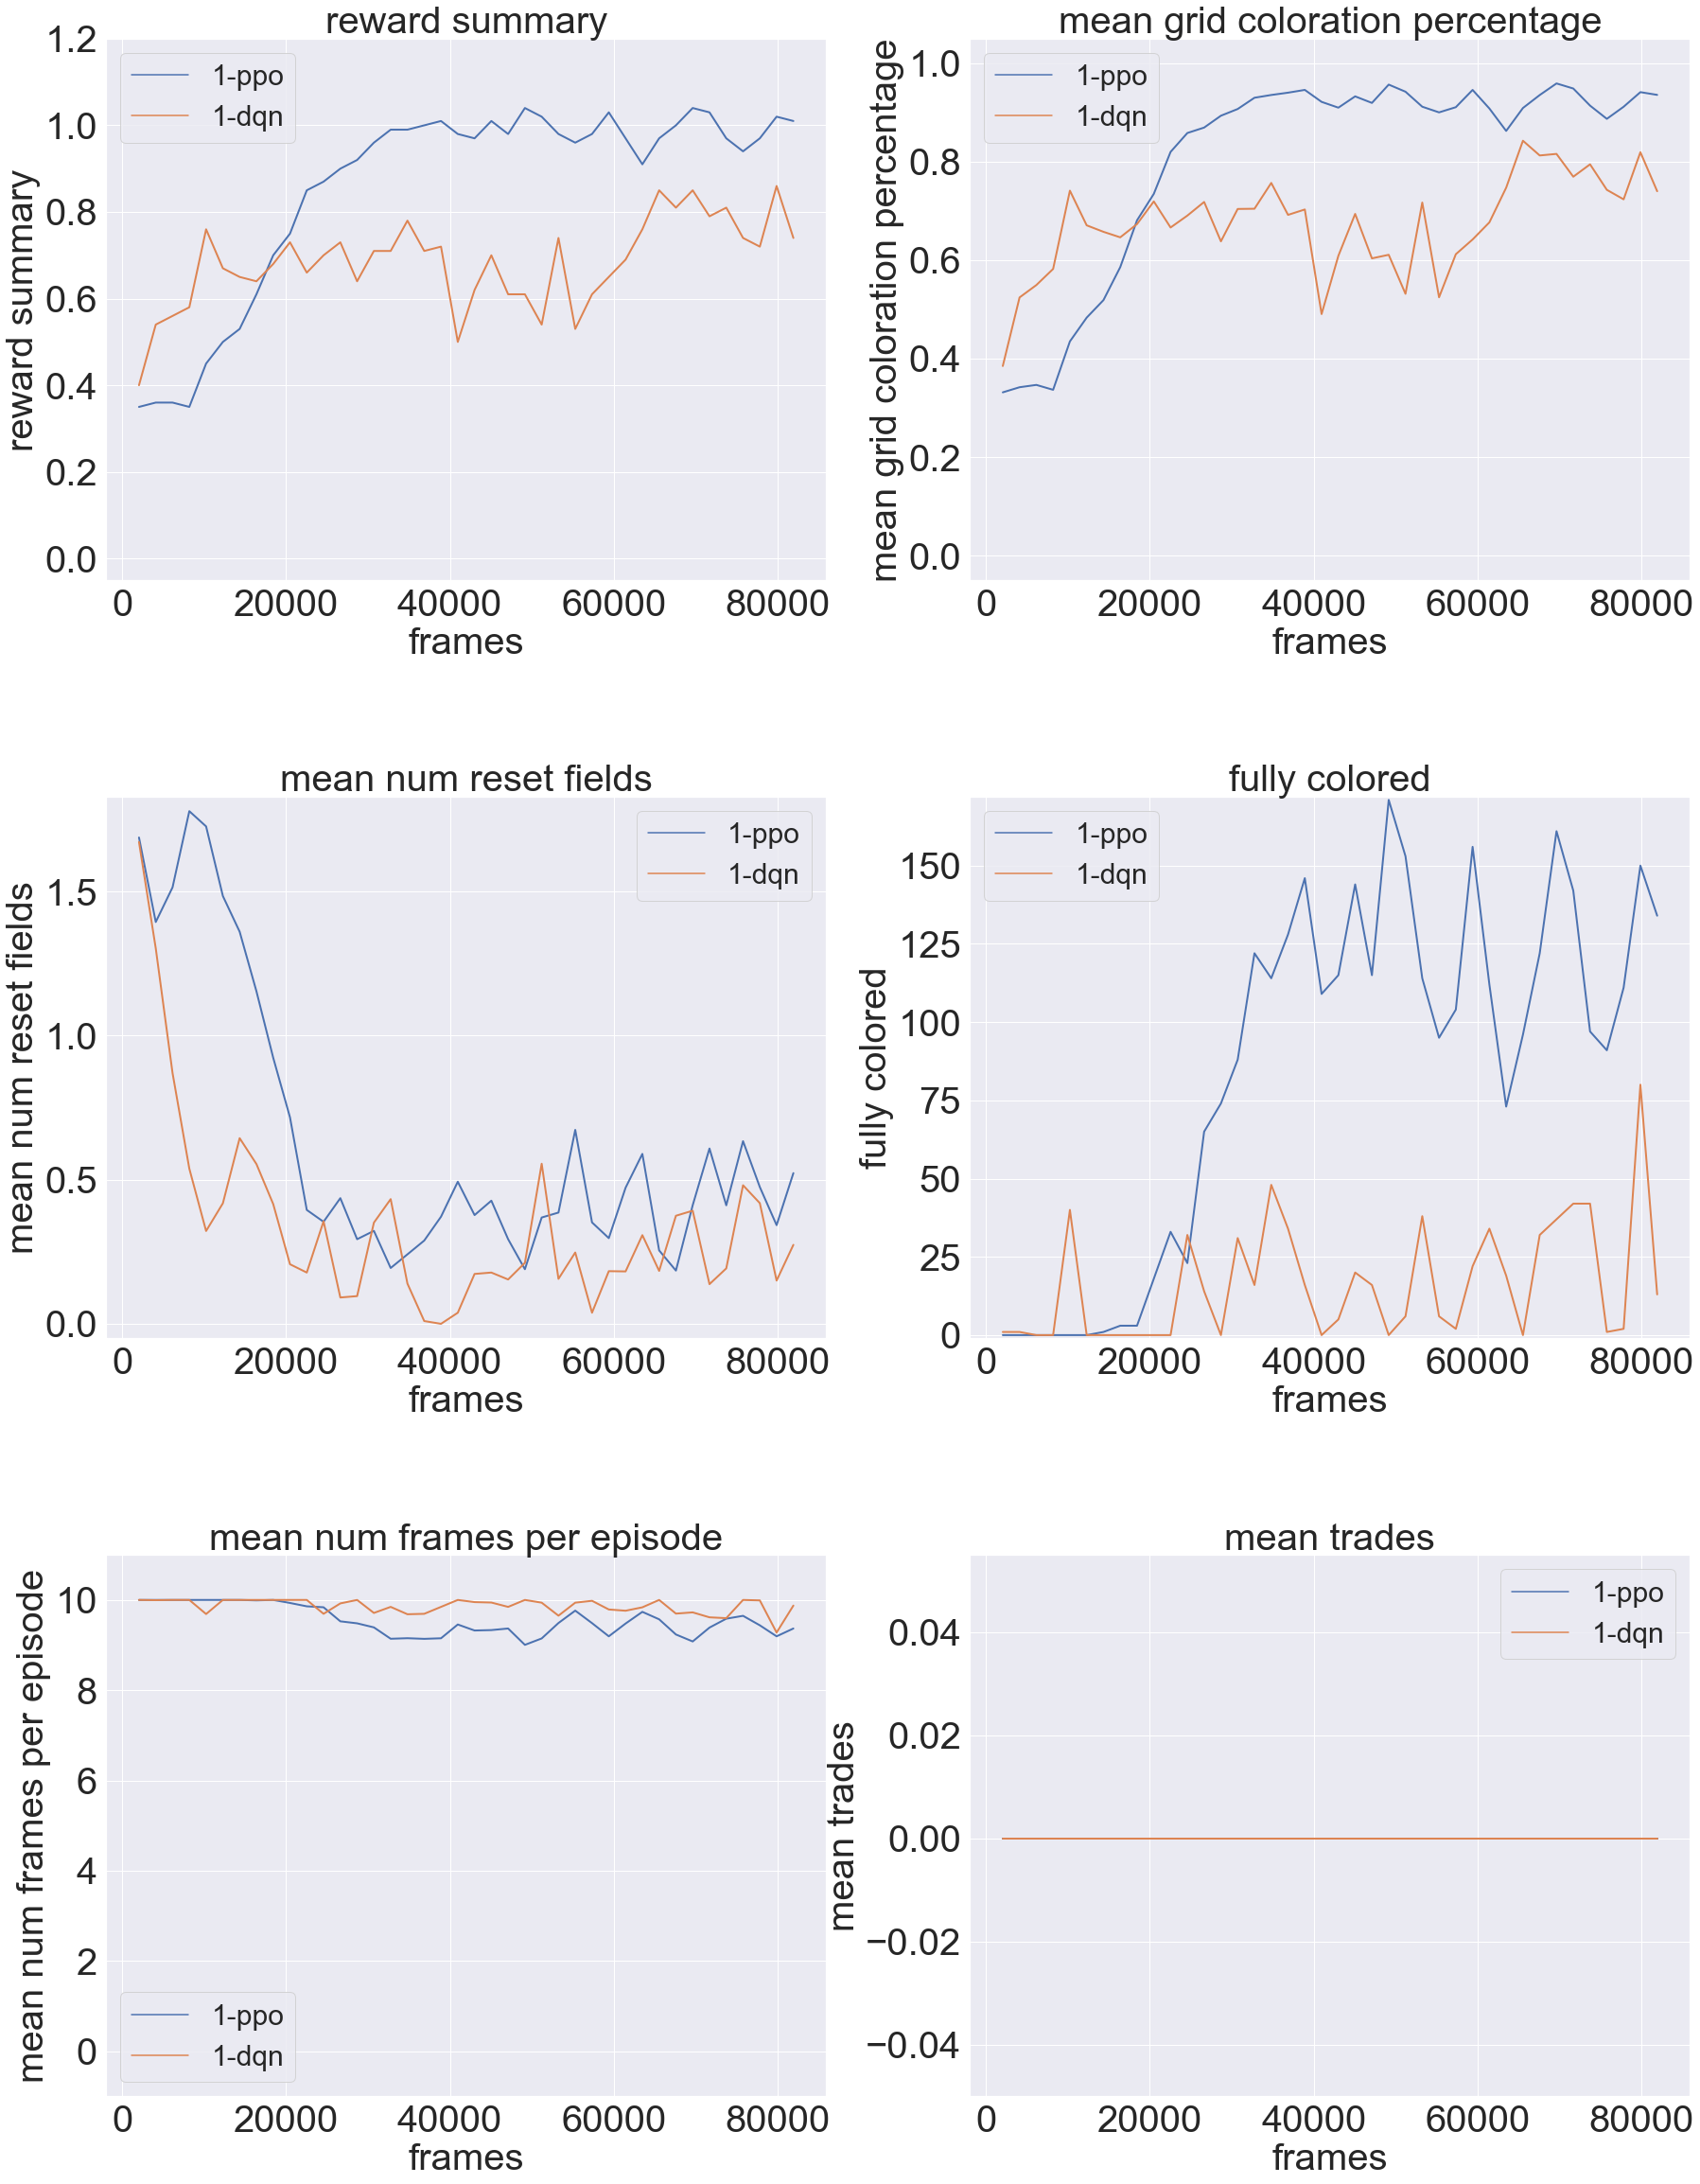
\includegraphics[width=1\textwidth]{AX-easy-1.png}\\
    \caption[PPO and DQN Training Details with One Agent]{Details of the training with one agent using PPO and DQN}\label{fig:ax-easy-1}
\end{figure}
\vfill
\clearpage


\newpage
\vfill
\begin{figure}
    \centering
    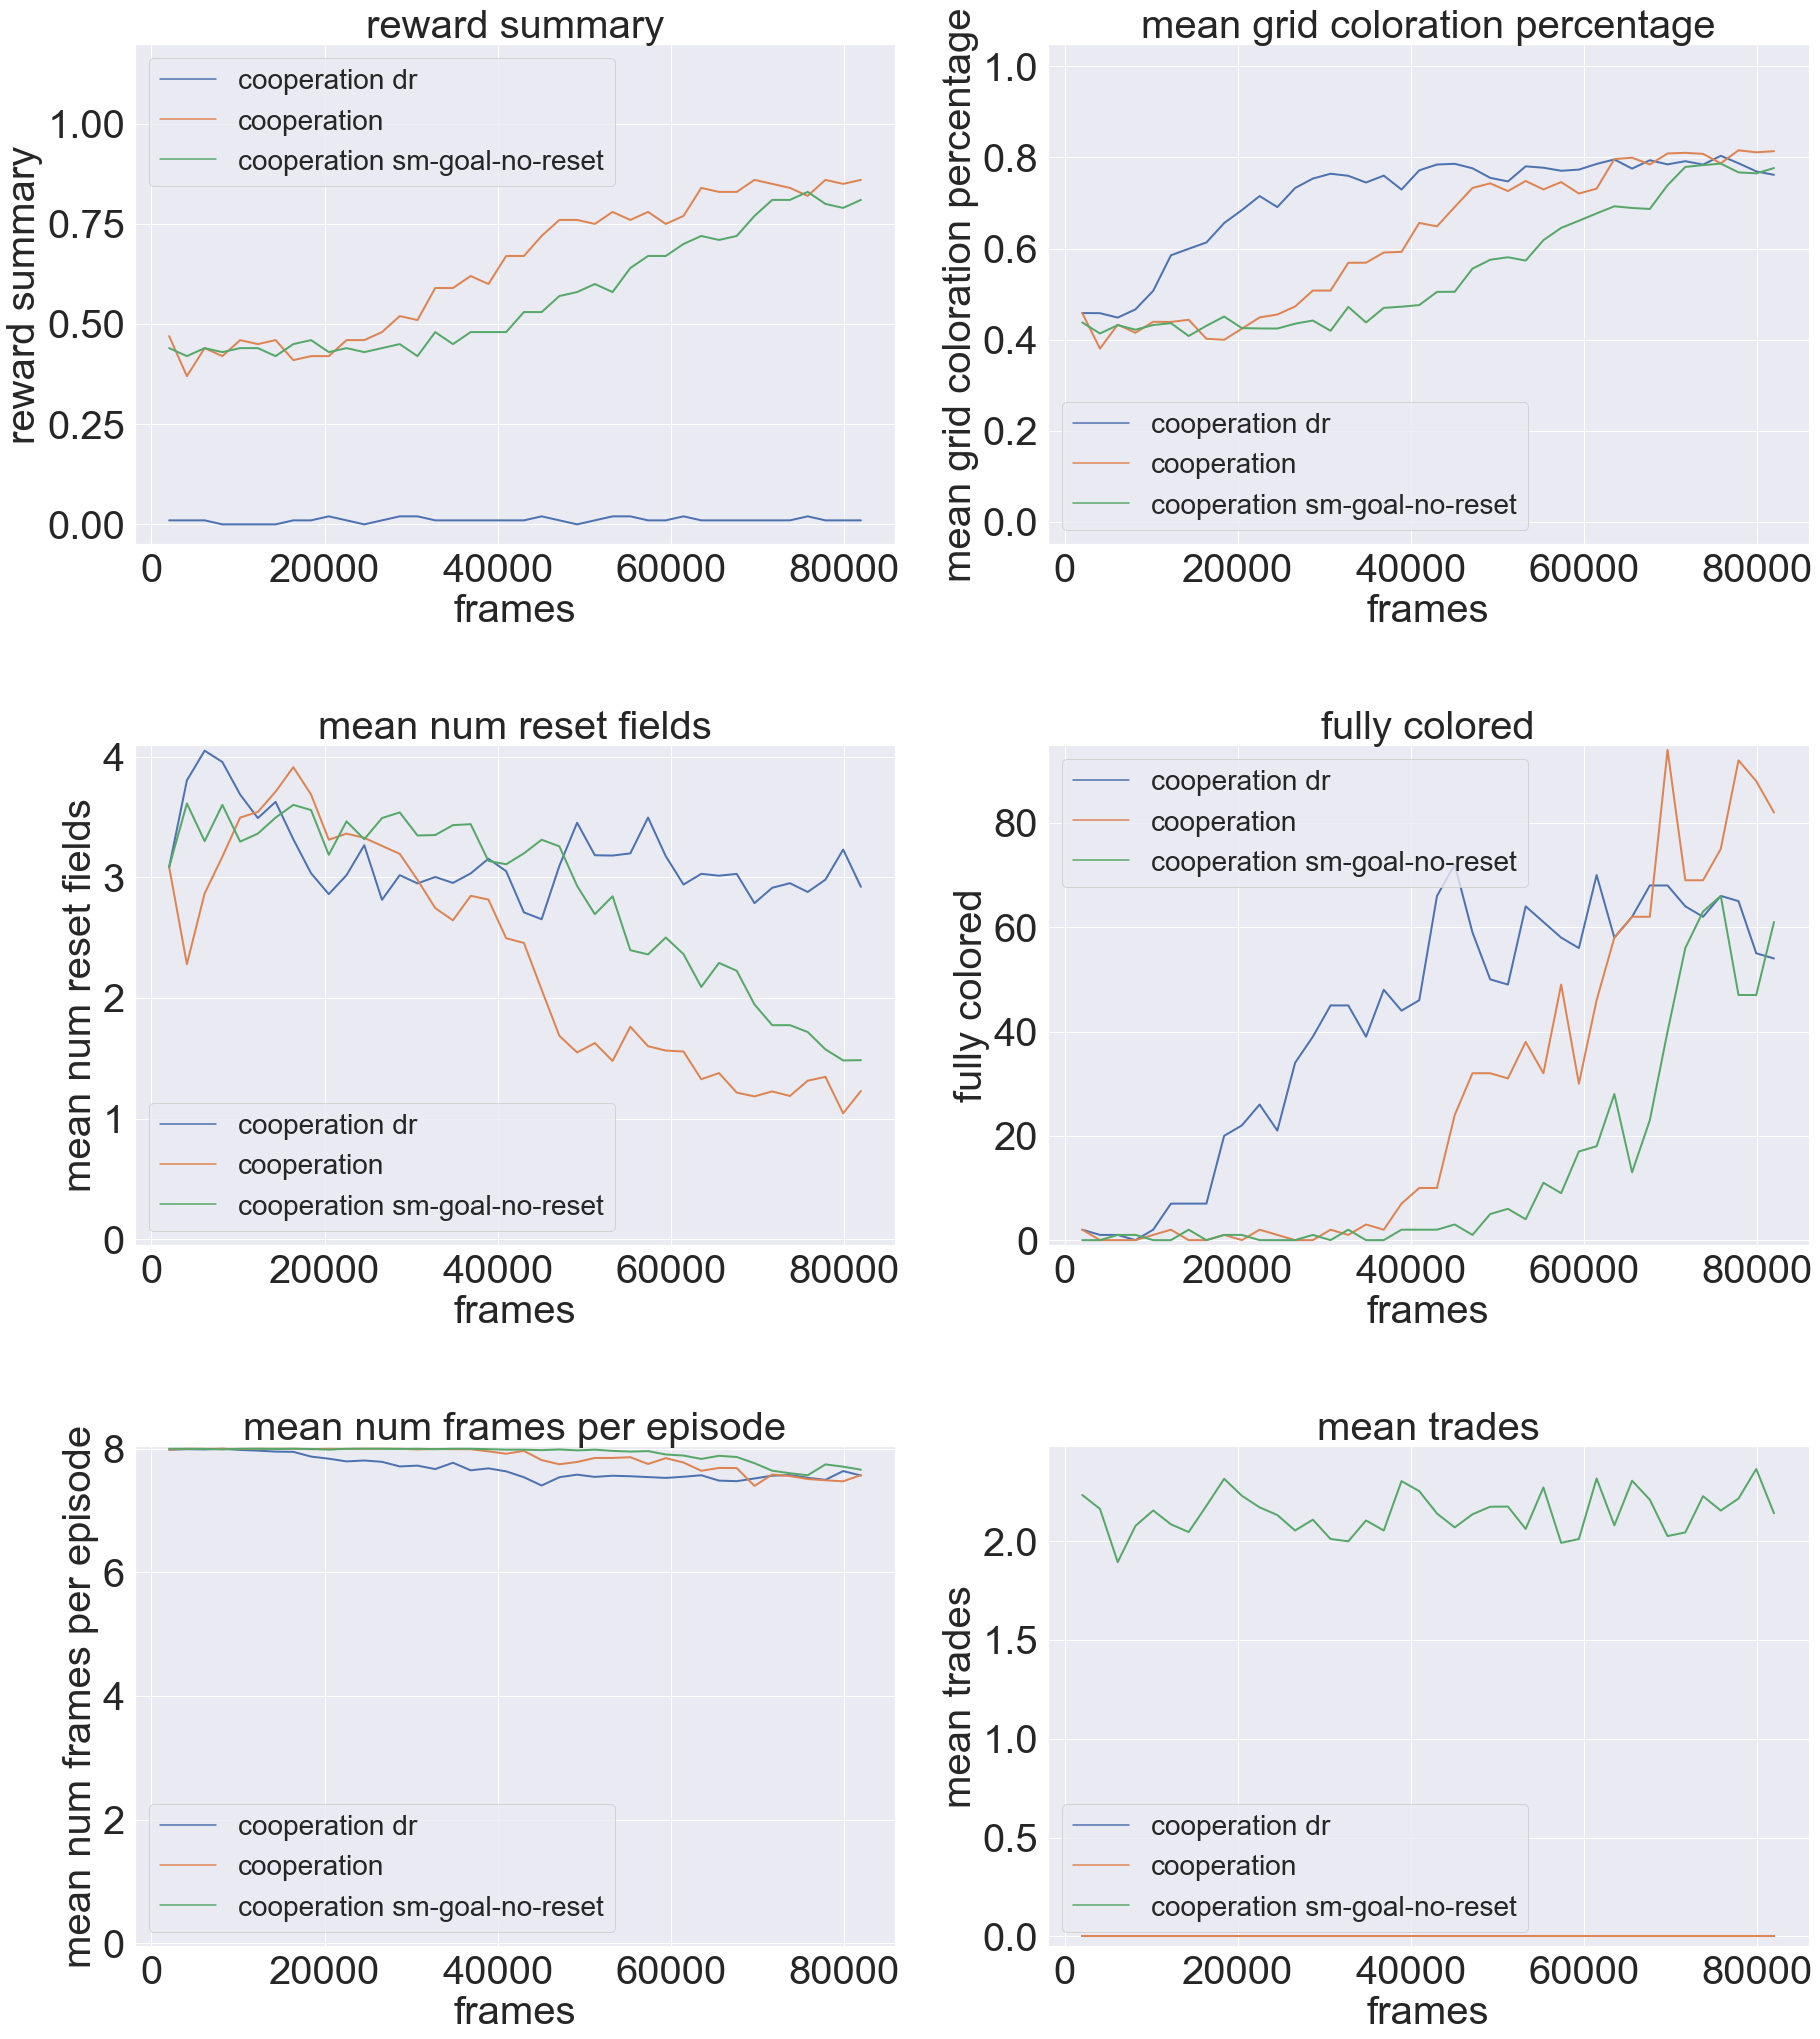
\includegraphics[width=1\textwidth]{AX-easy-2-ppo-coop.png}\\
    \caption[Training Details of Top PPO Cooperation Executions]{Top cooperation score details of two PPO agents}\label{fig:ax-easy-2-ppo-coop}
\end{figure}
\vfill
\clearpage


\newpage
\vfill
\begin{figure}
    \centering
    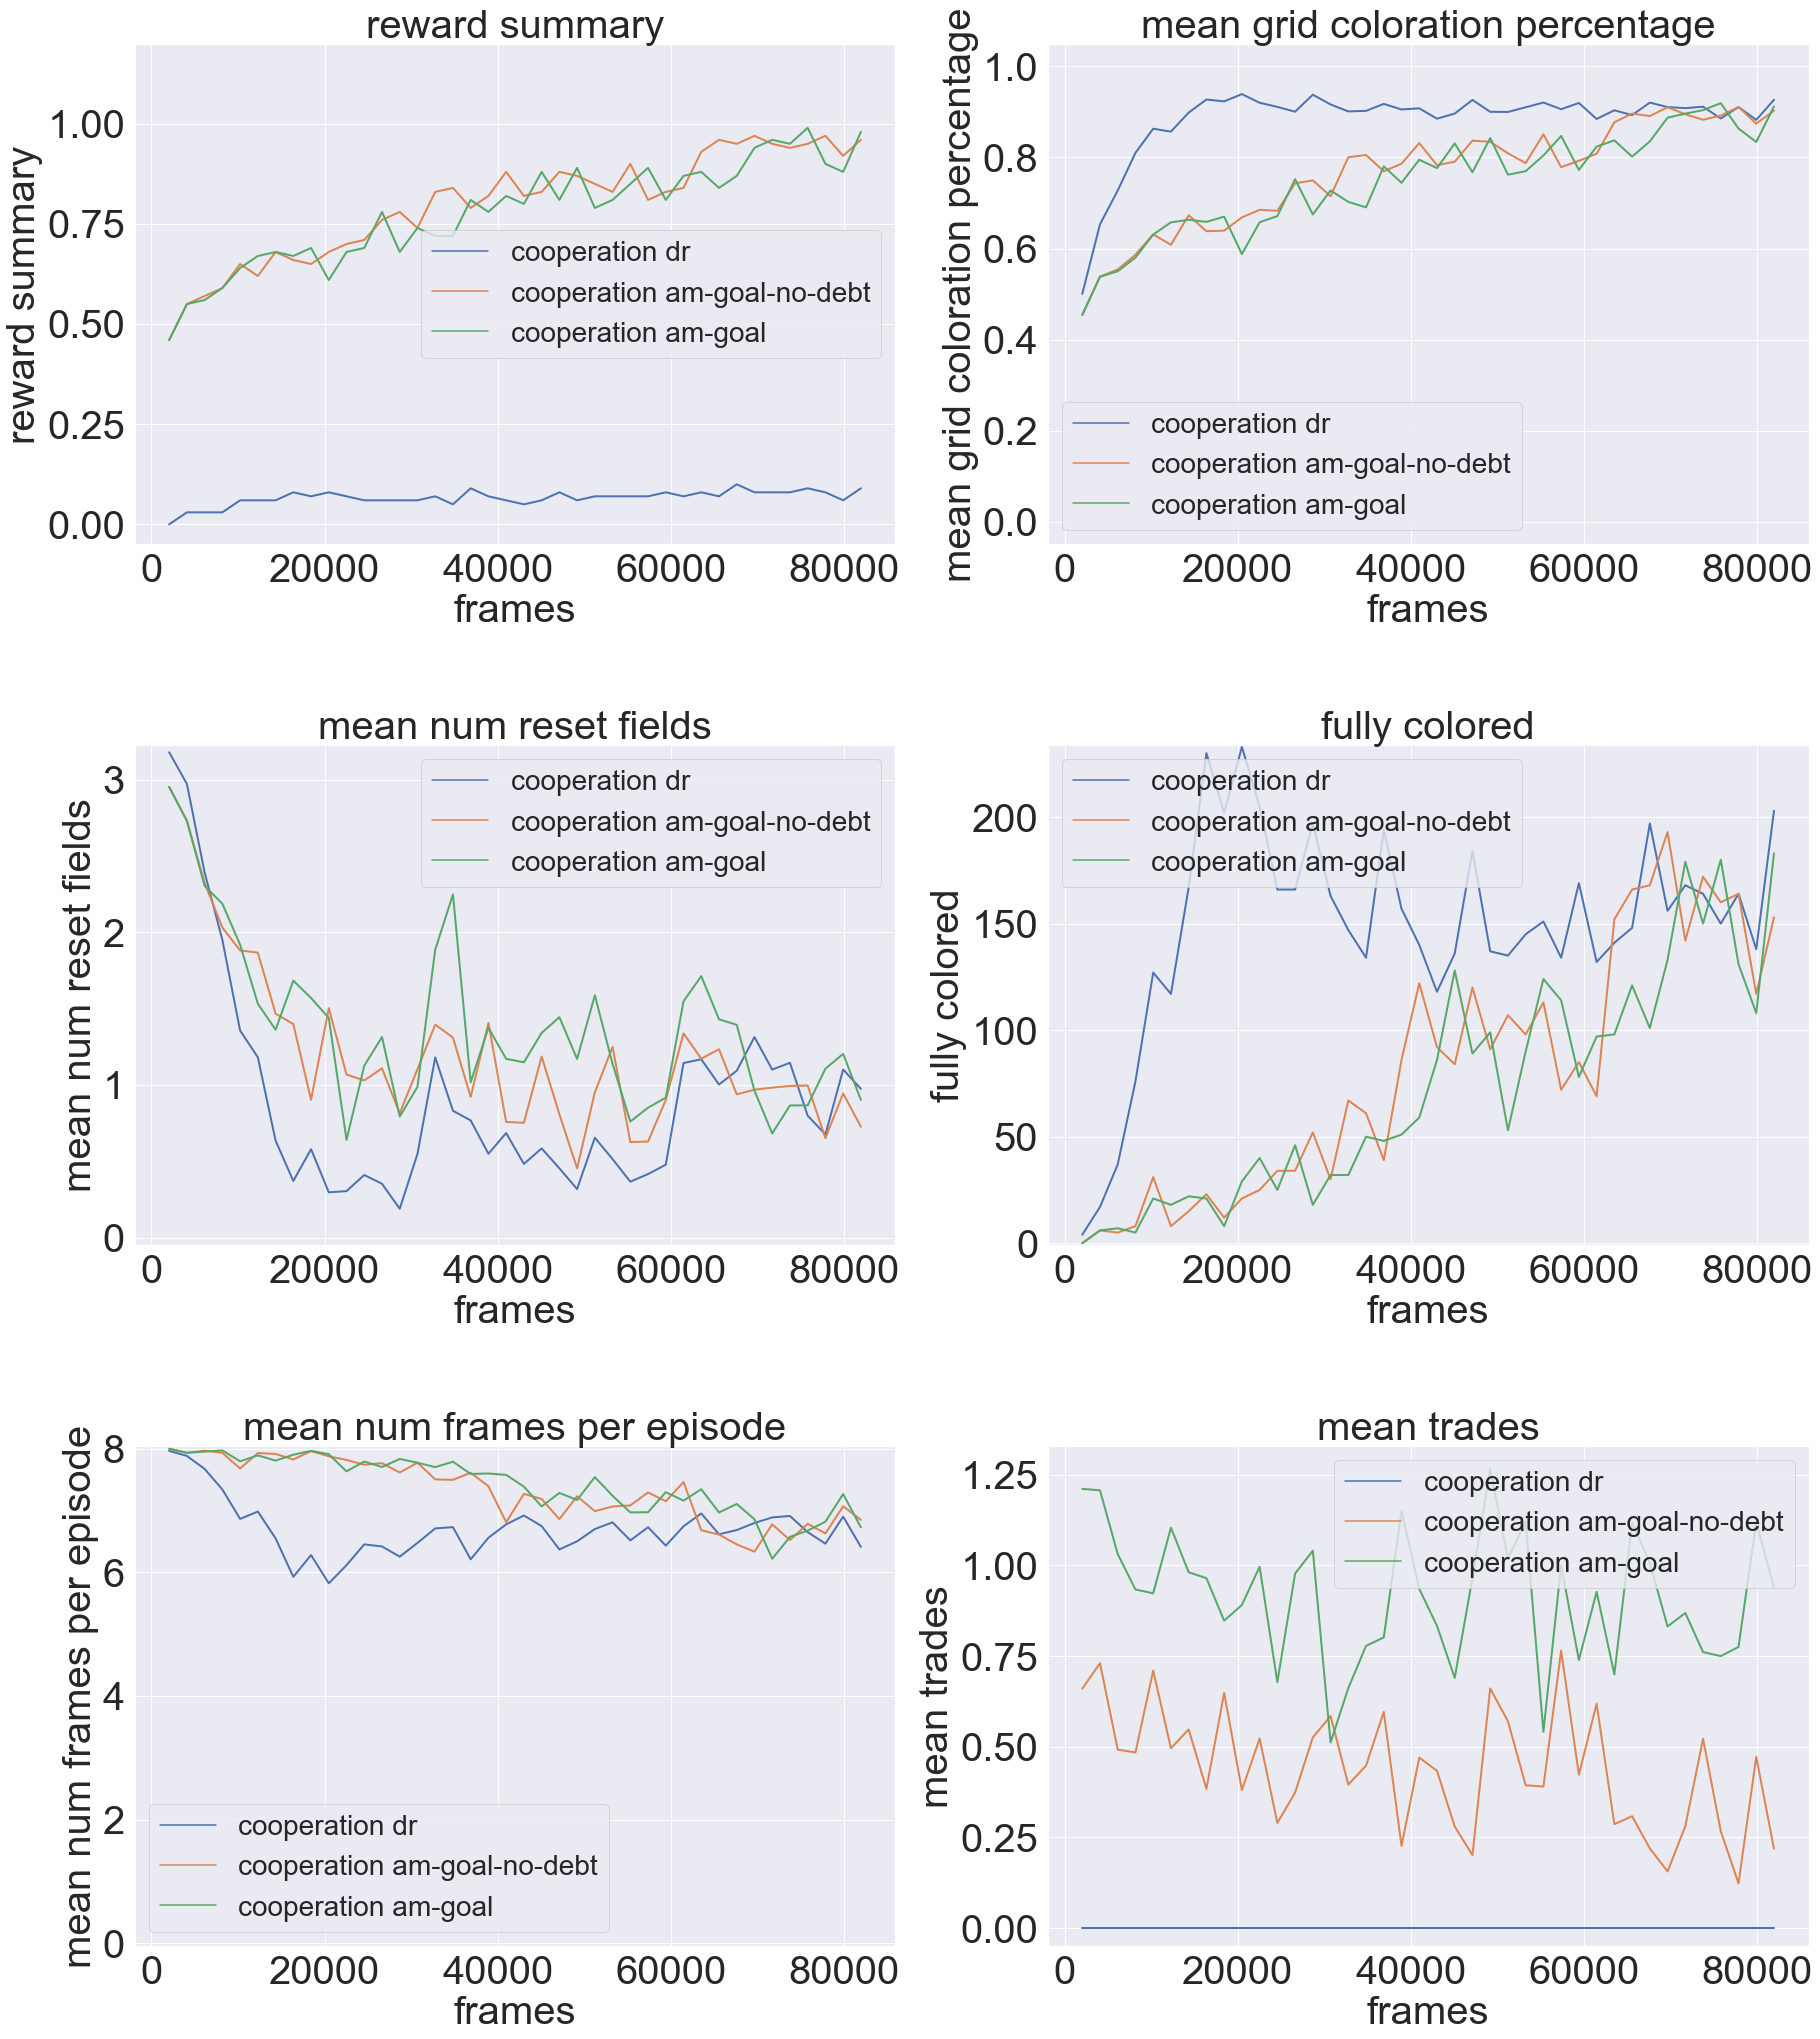
\includegraphics[width=1\textwidth]{AX-easy-2-dqn-coop.png}\\
    \caption[Training Details of Top DQN Cooperation Executions]{Top cooperation score details of two DQN agents}\label{fig:ax-easy-2-dqn-coop}
\end{figure}
\vfill
\clearpage


\newpage
\vfill
\begin{figure}
    \centering
    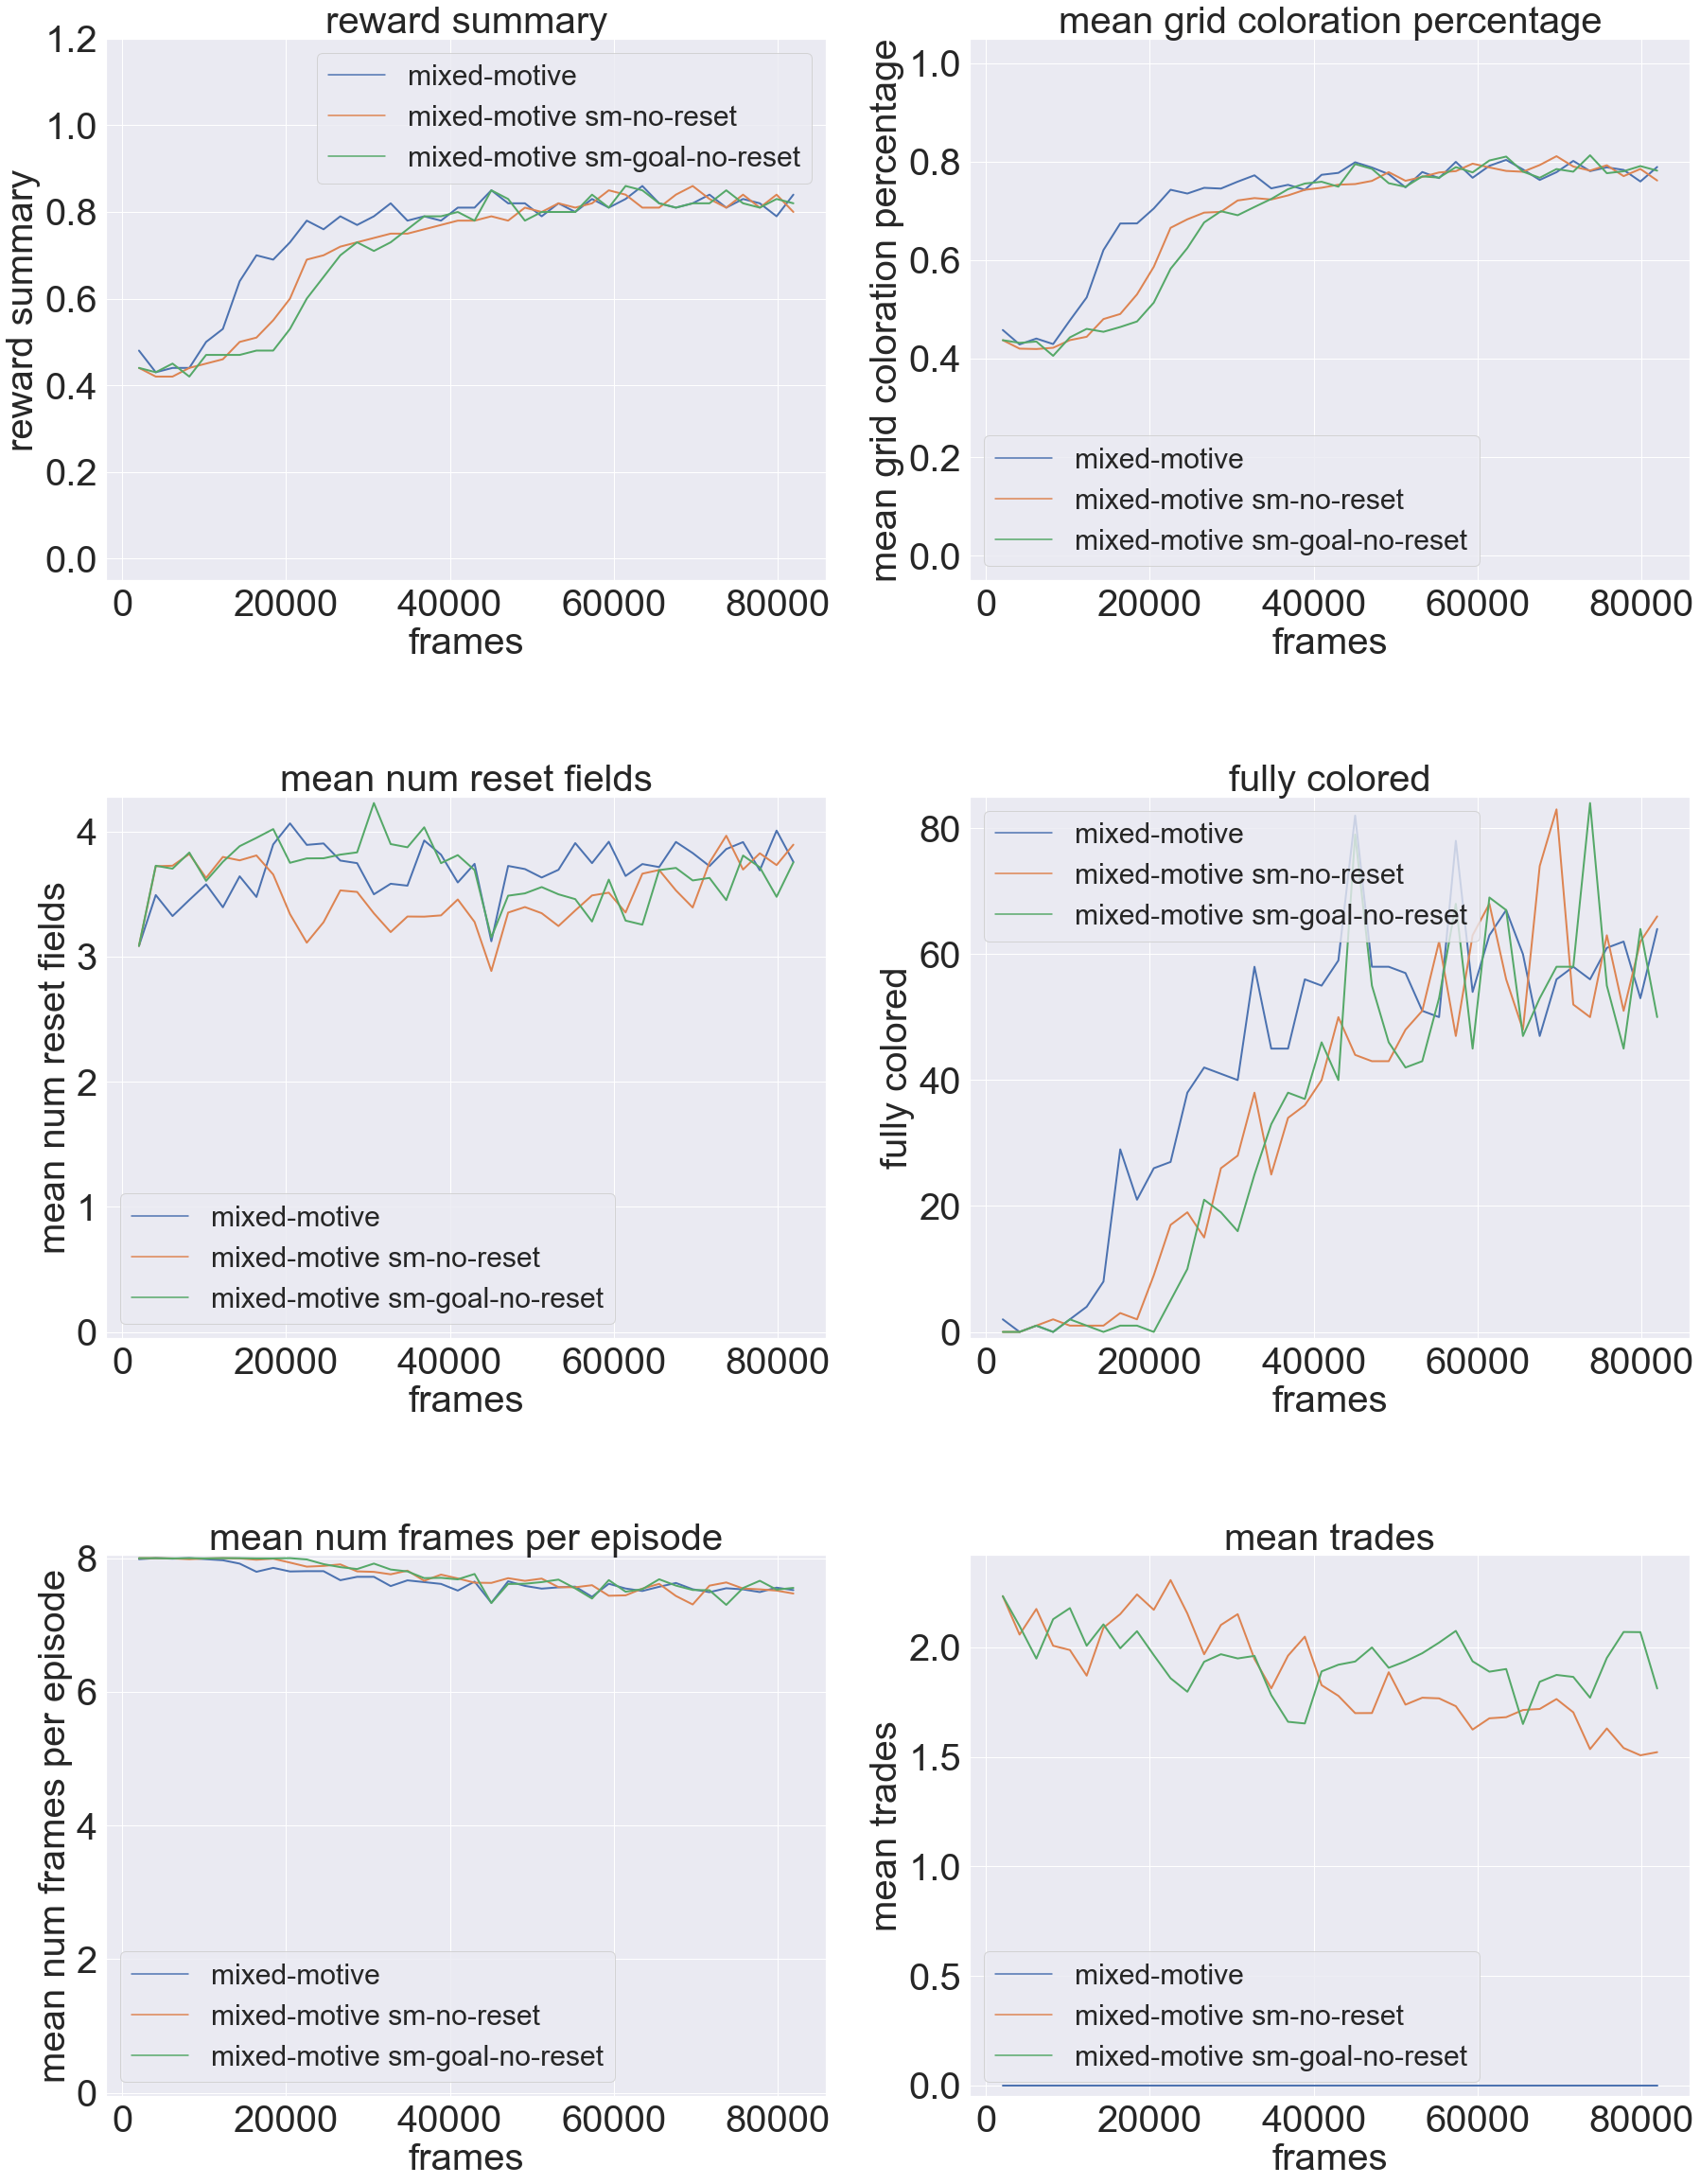
\includegraphics[width=1\textwidth]{AX-easy-2-ppo-mixed.png}\\
    \caption[Training Details of Top PPO Mixed-Motive Executions]{Top mixed-motive score details of two PPO agents}\label{fig:ax-easy-2-ppo-mixed}
\end{figure}
\vfill
\clearpage


\newpage
\vfill
\begin{figure}
    \centering
    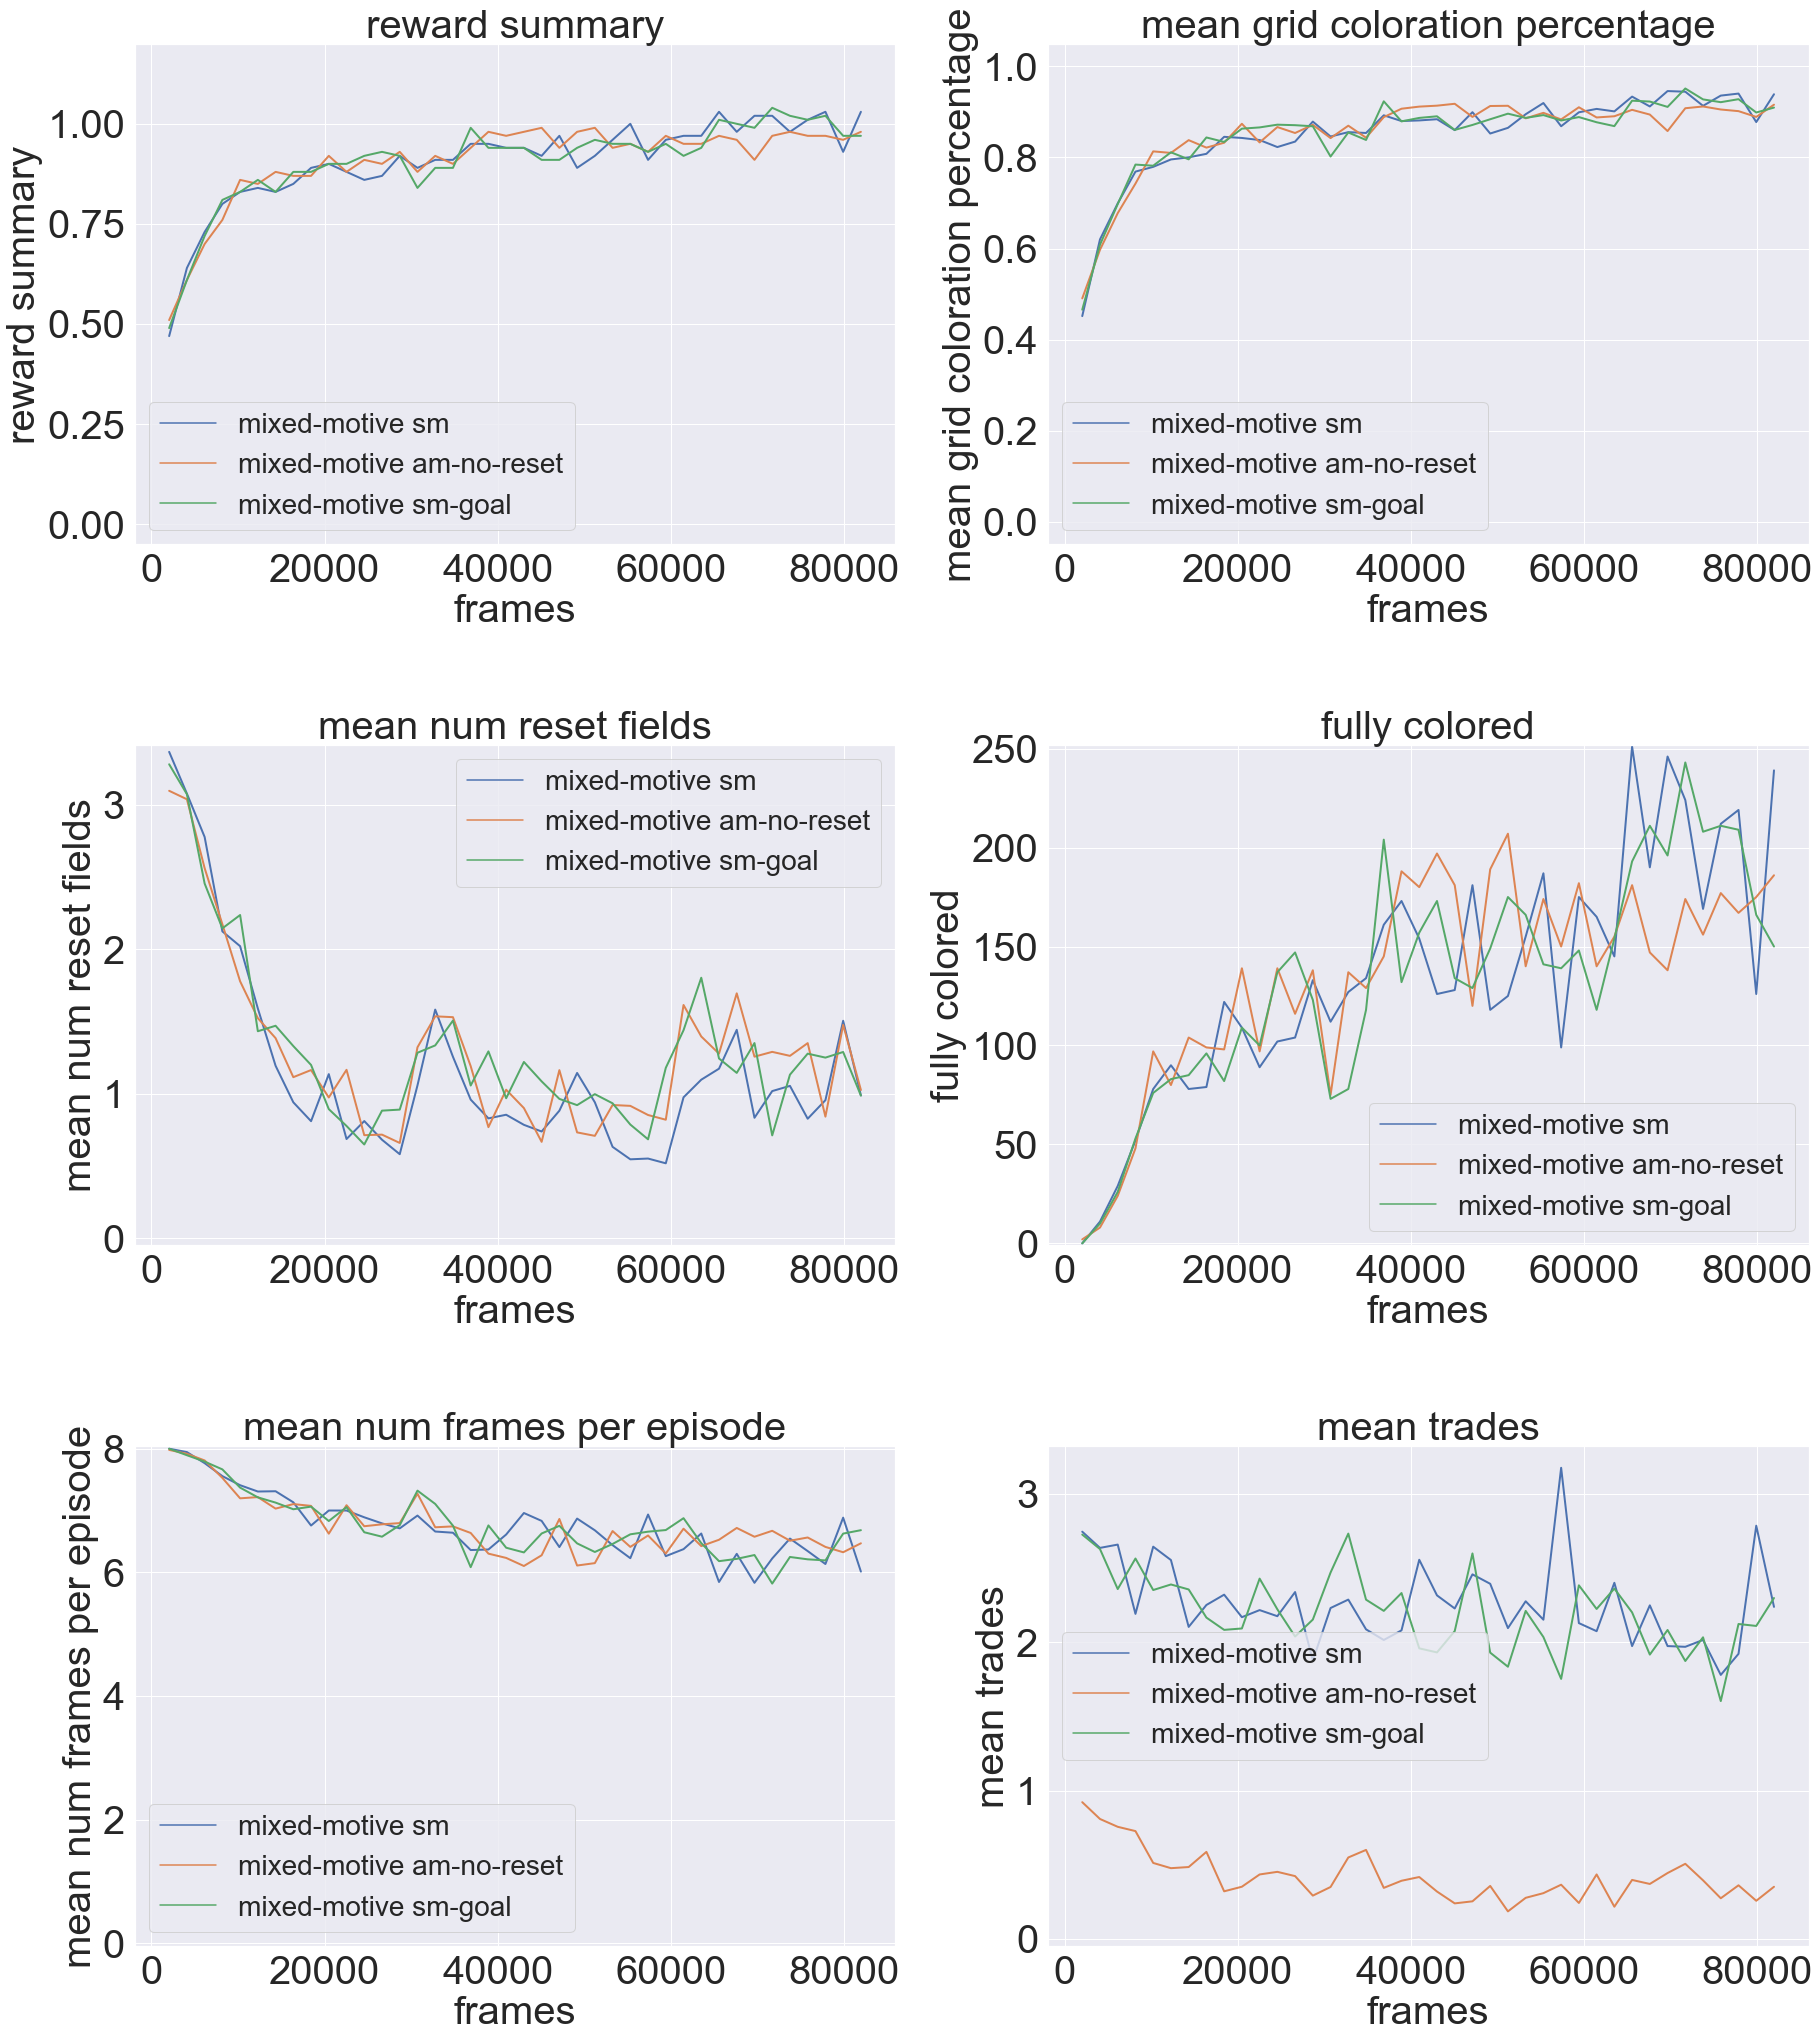
\includegraphics[width=1\textwidth]{AX-easy-2-dqn-mixed.png}\\
    \caption[Training Details of Top DQN Mixed-Motive Executions]{Top mixed-motive score details of two DQN agents}\label{fig:ax-easy-2-dqn-mixed}
\end{figure}
\vfill
\clearpage


\newpage
\vfill
\begin{figure}
    \centering
    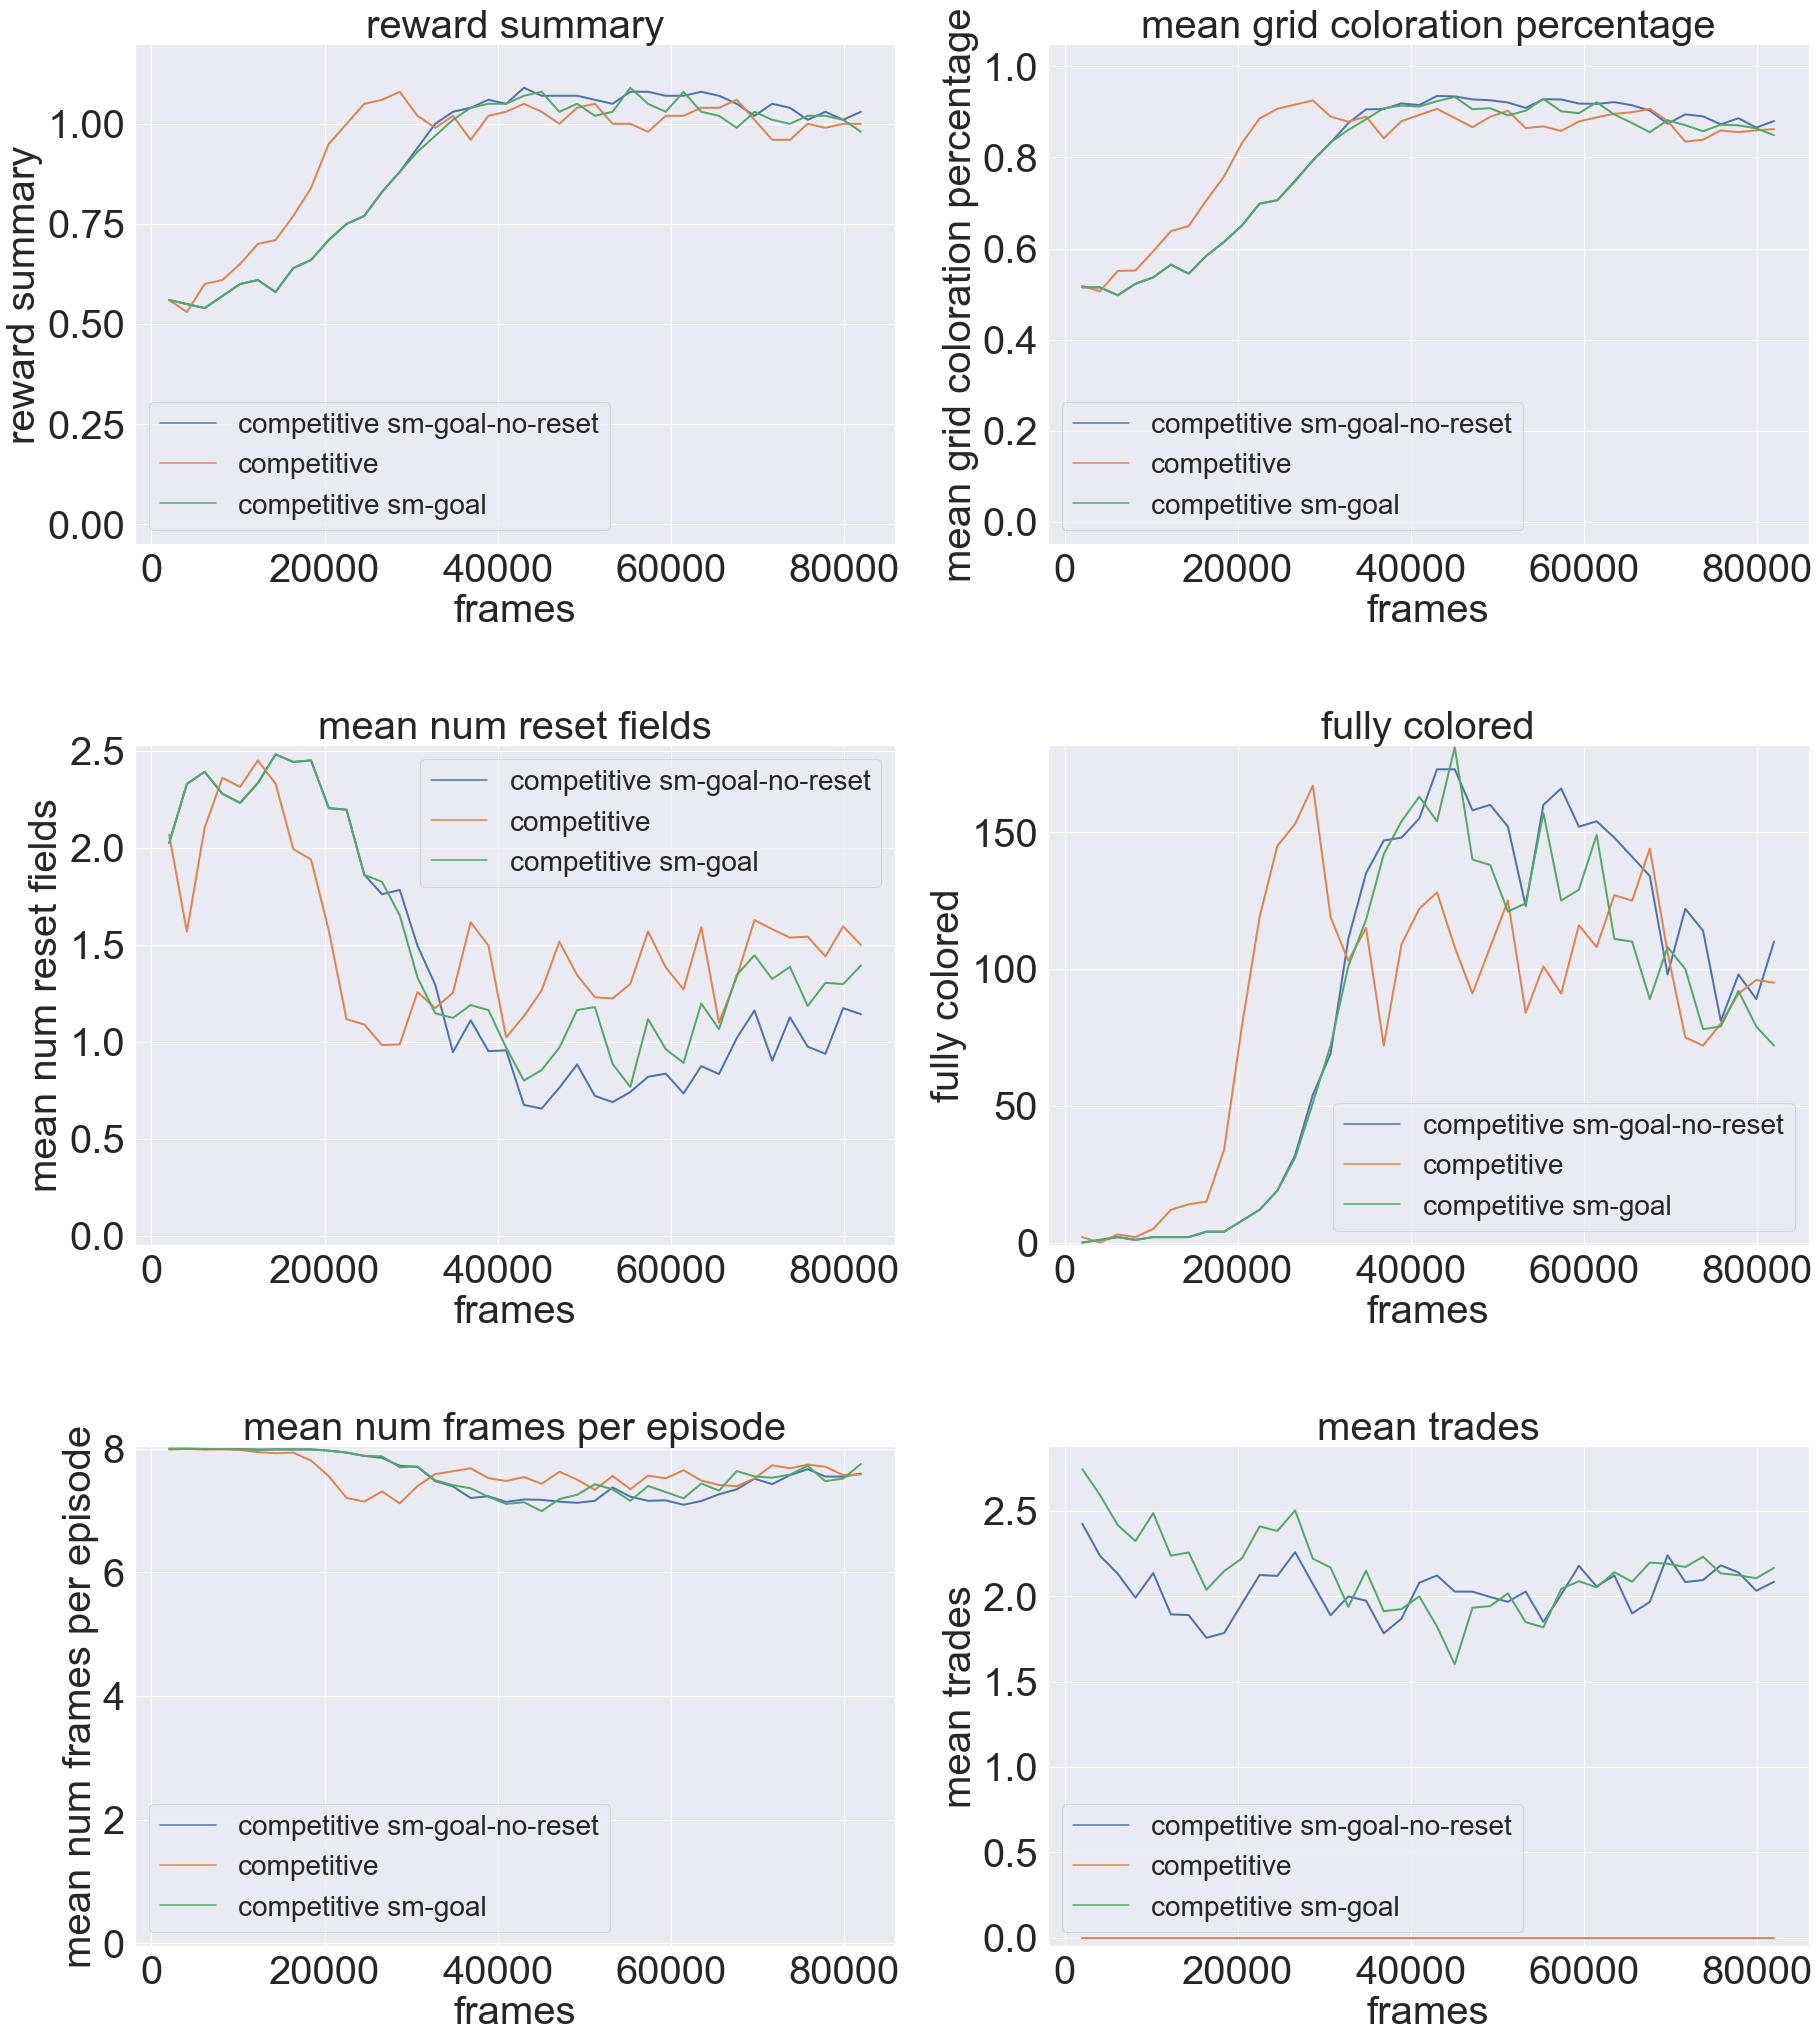
\includegraphics[width=1\textwidth]{AX-easy-2-ppo-comp.png}\\
    \caption[Training Details of Top PPO Competitive Executions]{Top competitive score details of two PPO agents}\label{fig:ax-easy-2-ppo-comp}
\end{figure}
\vfill
\clearpage


\newpage
\vfill
\begin{figure}
    \centering
    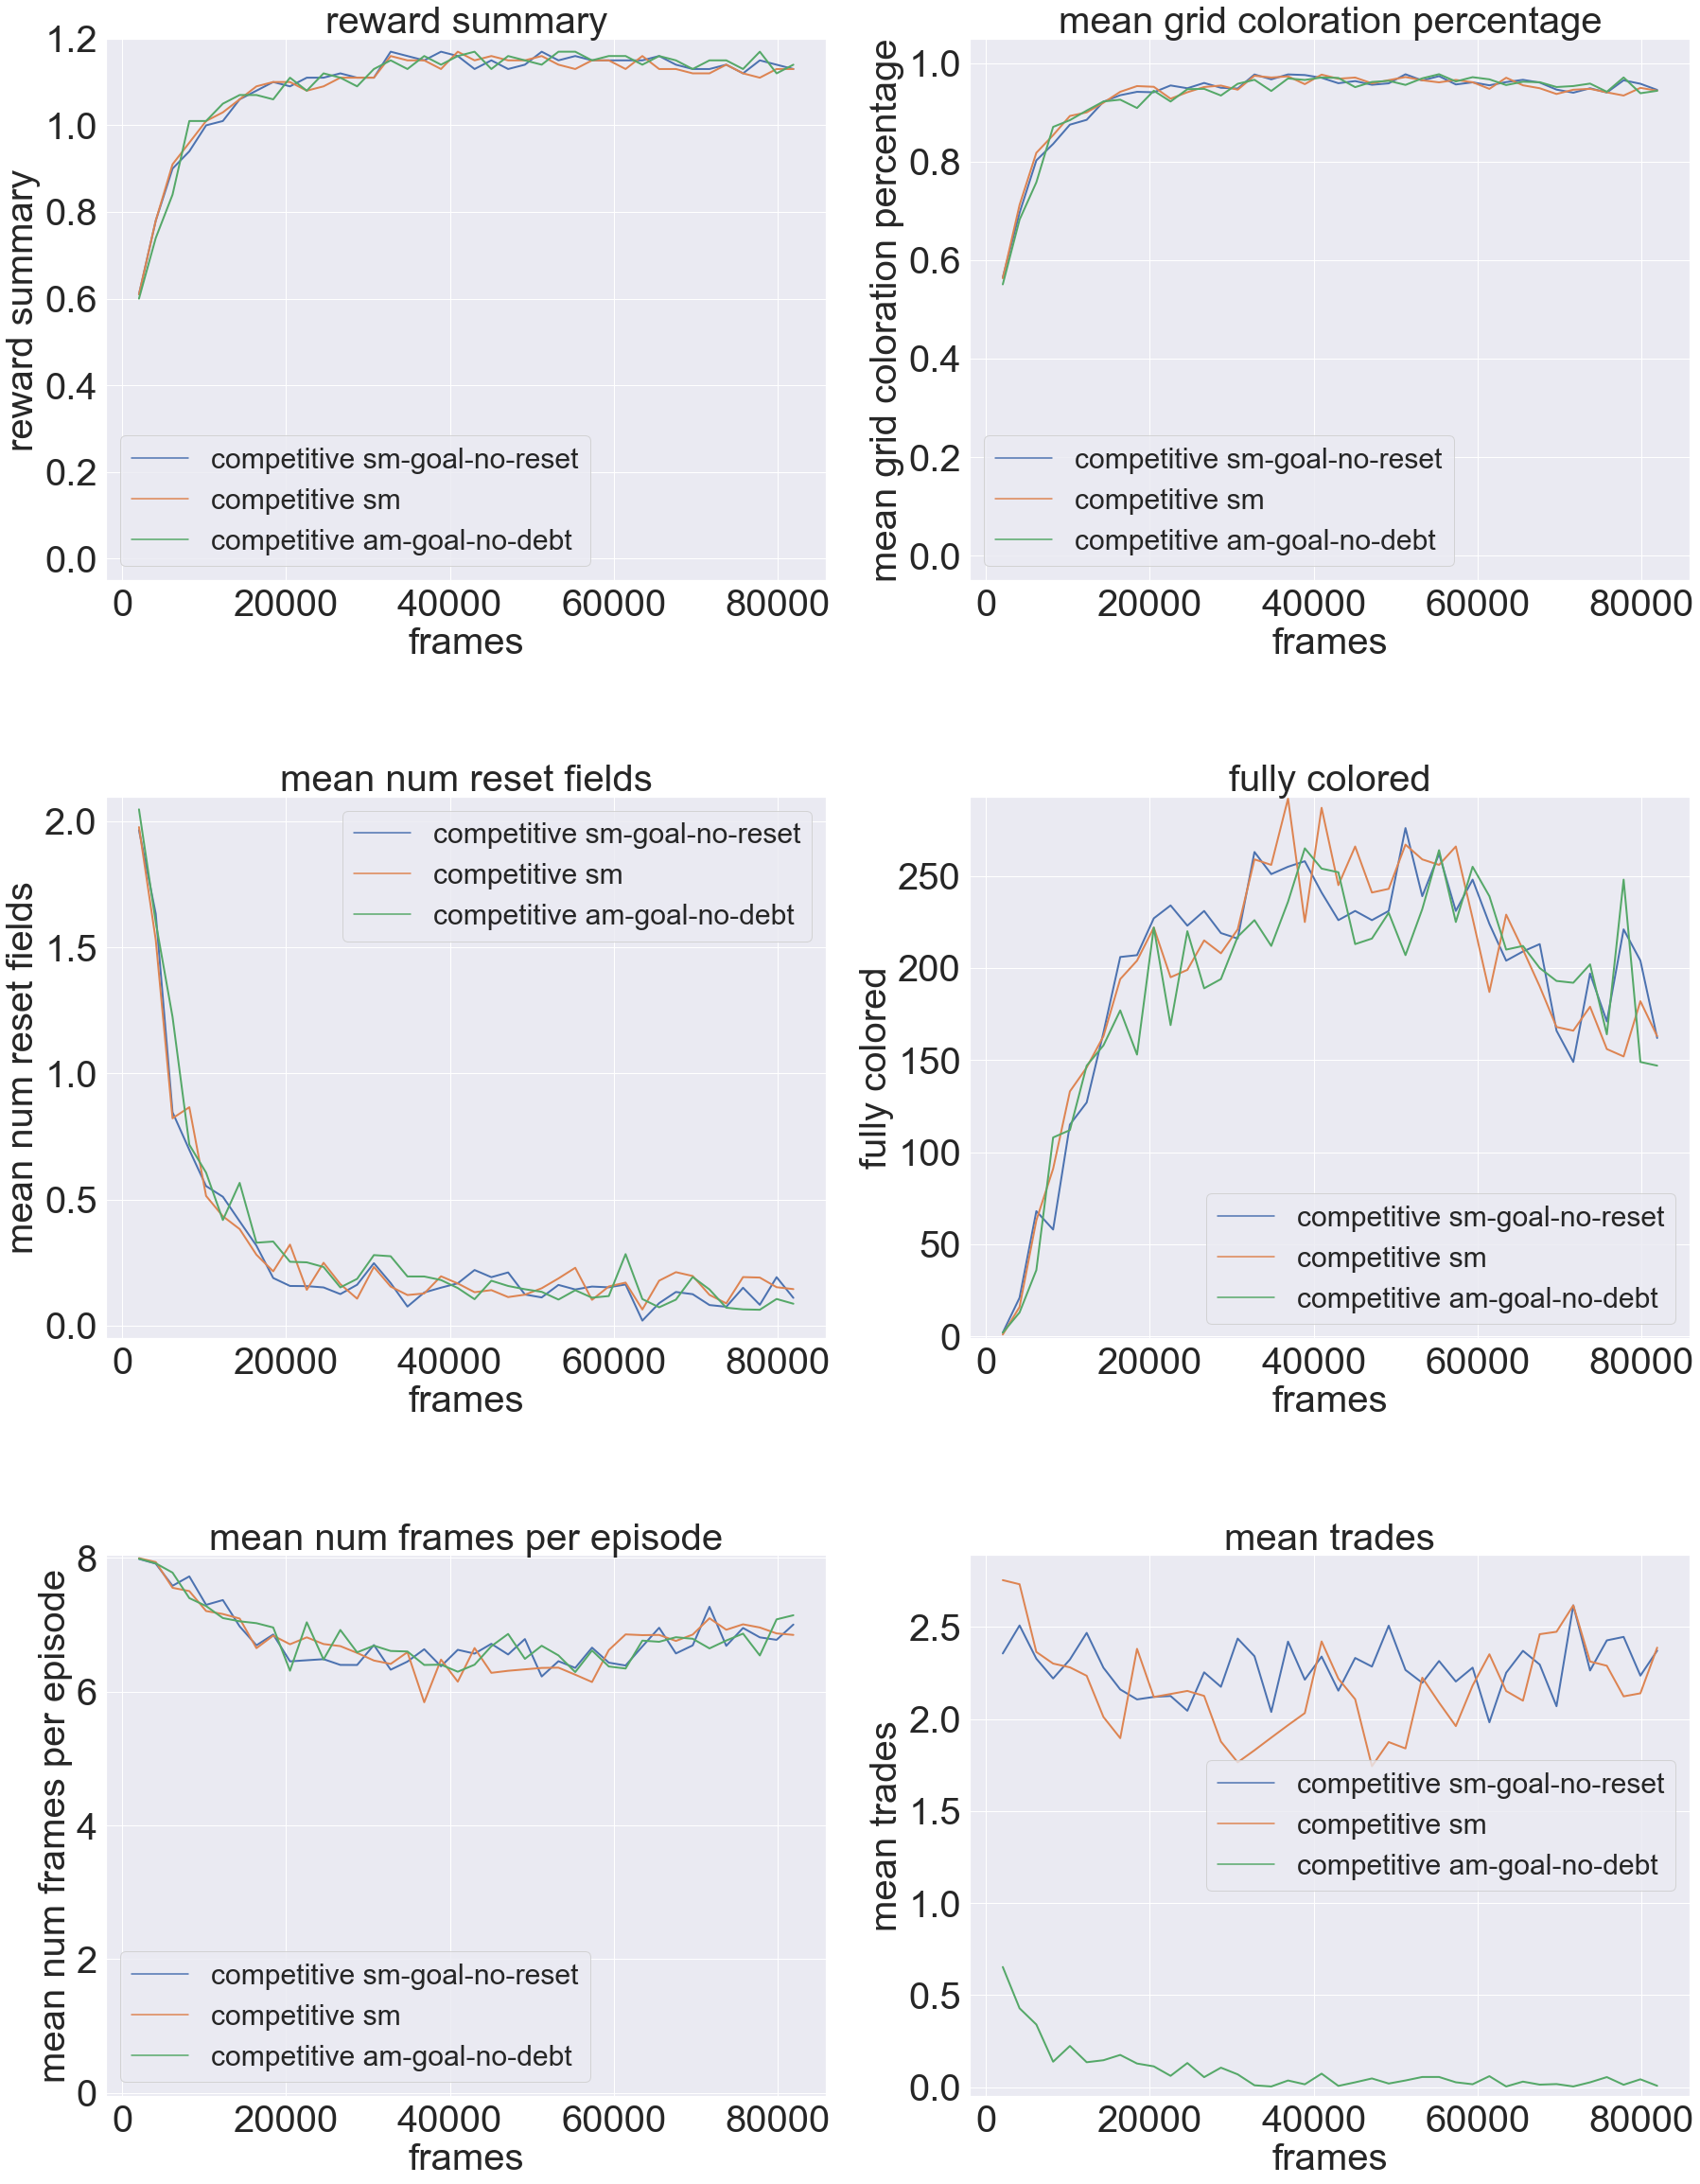
\includegraphics[width=1\textwidth]{AX-easy-2-dqn-comp.png}\\
    \caption[Training Details of Top DQN Competitive Executions]{Top competitive score details of two DQN agents}\label{fig:ax-easy-2-dqn-comp}
\end{figure}
\vfill
\clearpage

\subsection{Difficult Environment}
An example to run a training process in a seven by seven environment is shown below.

\begin{lstlisting}[float=htp,language=bash, escapeinside={//@}{@//},xleftmargin=3ex,xrightmargin=1ex]
$ python -m scripts.train 
    --algo dqn 
    --model dqn-difficult
    --agents 3
    --target-update 10000 
    --replay-size 700000 
    --epsilon-decay 20000
    --grid-size 7 
    --max-steps 20 
    --frames-per-proc 256
    --frames 200000
\end{lstlisting}

\newpage
\vfill
\begin{figure}
    \centering
    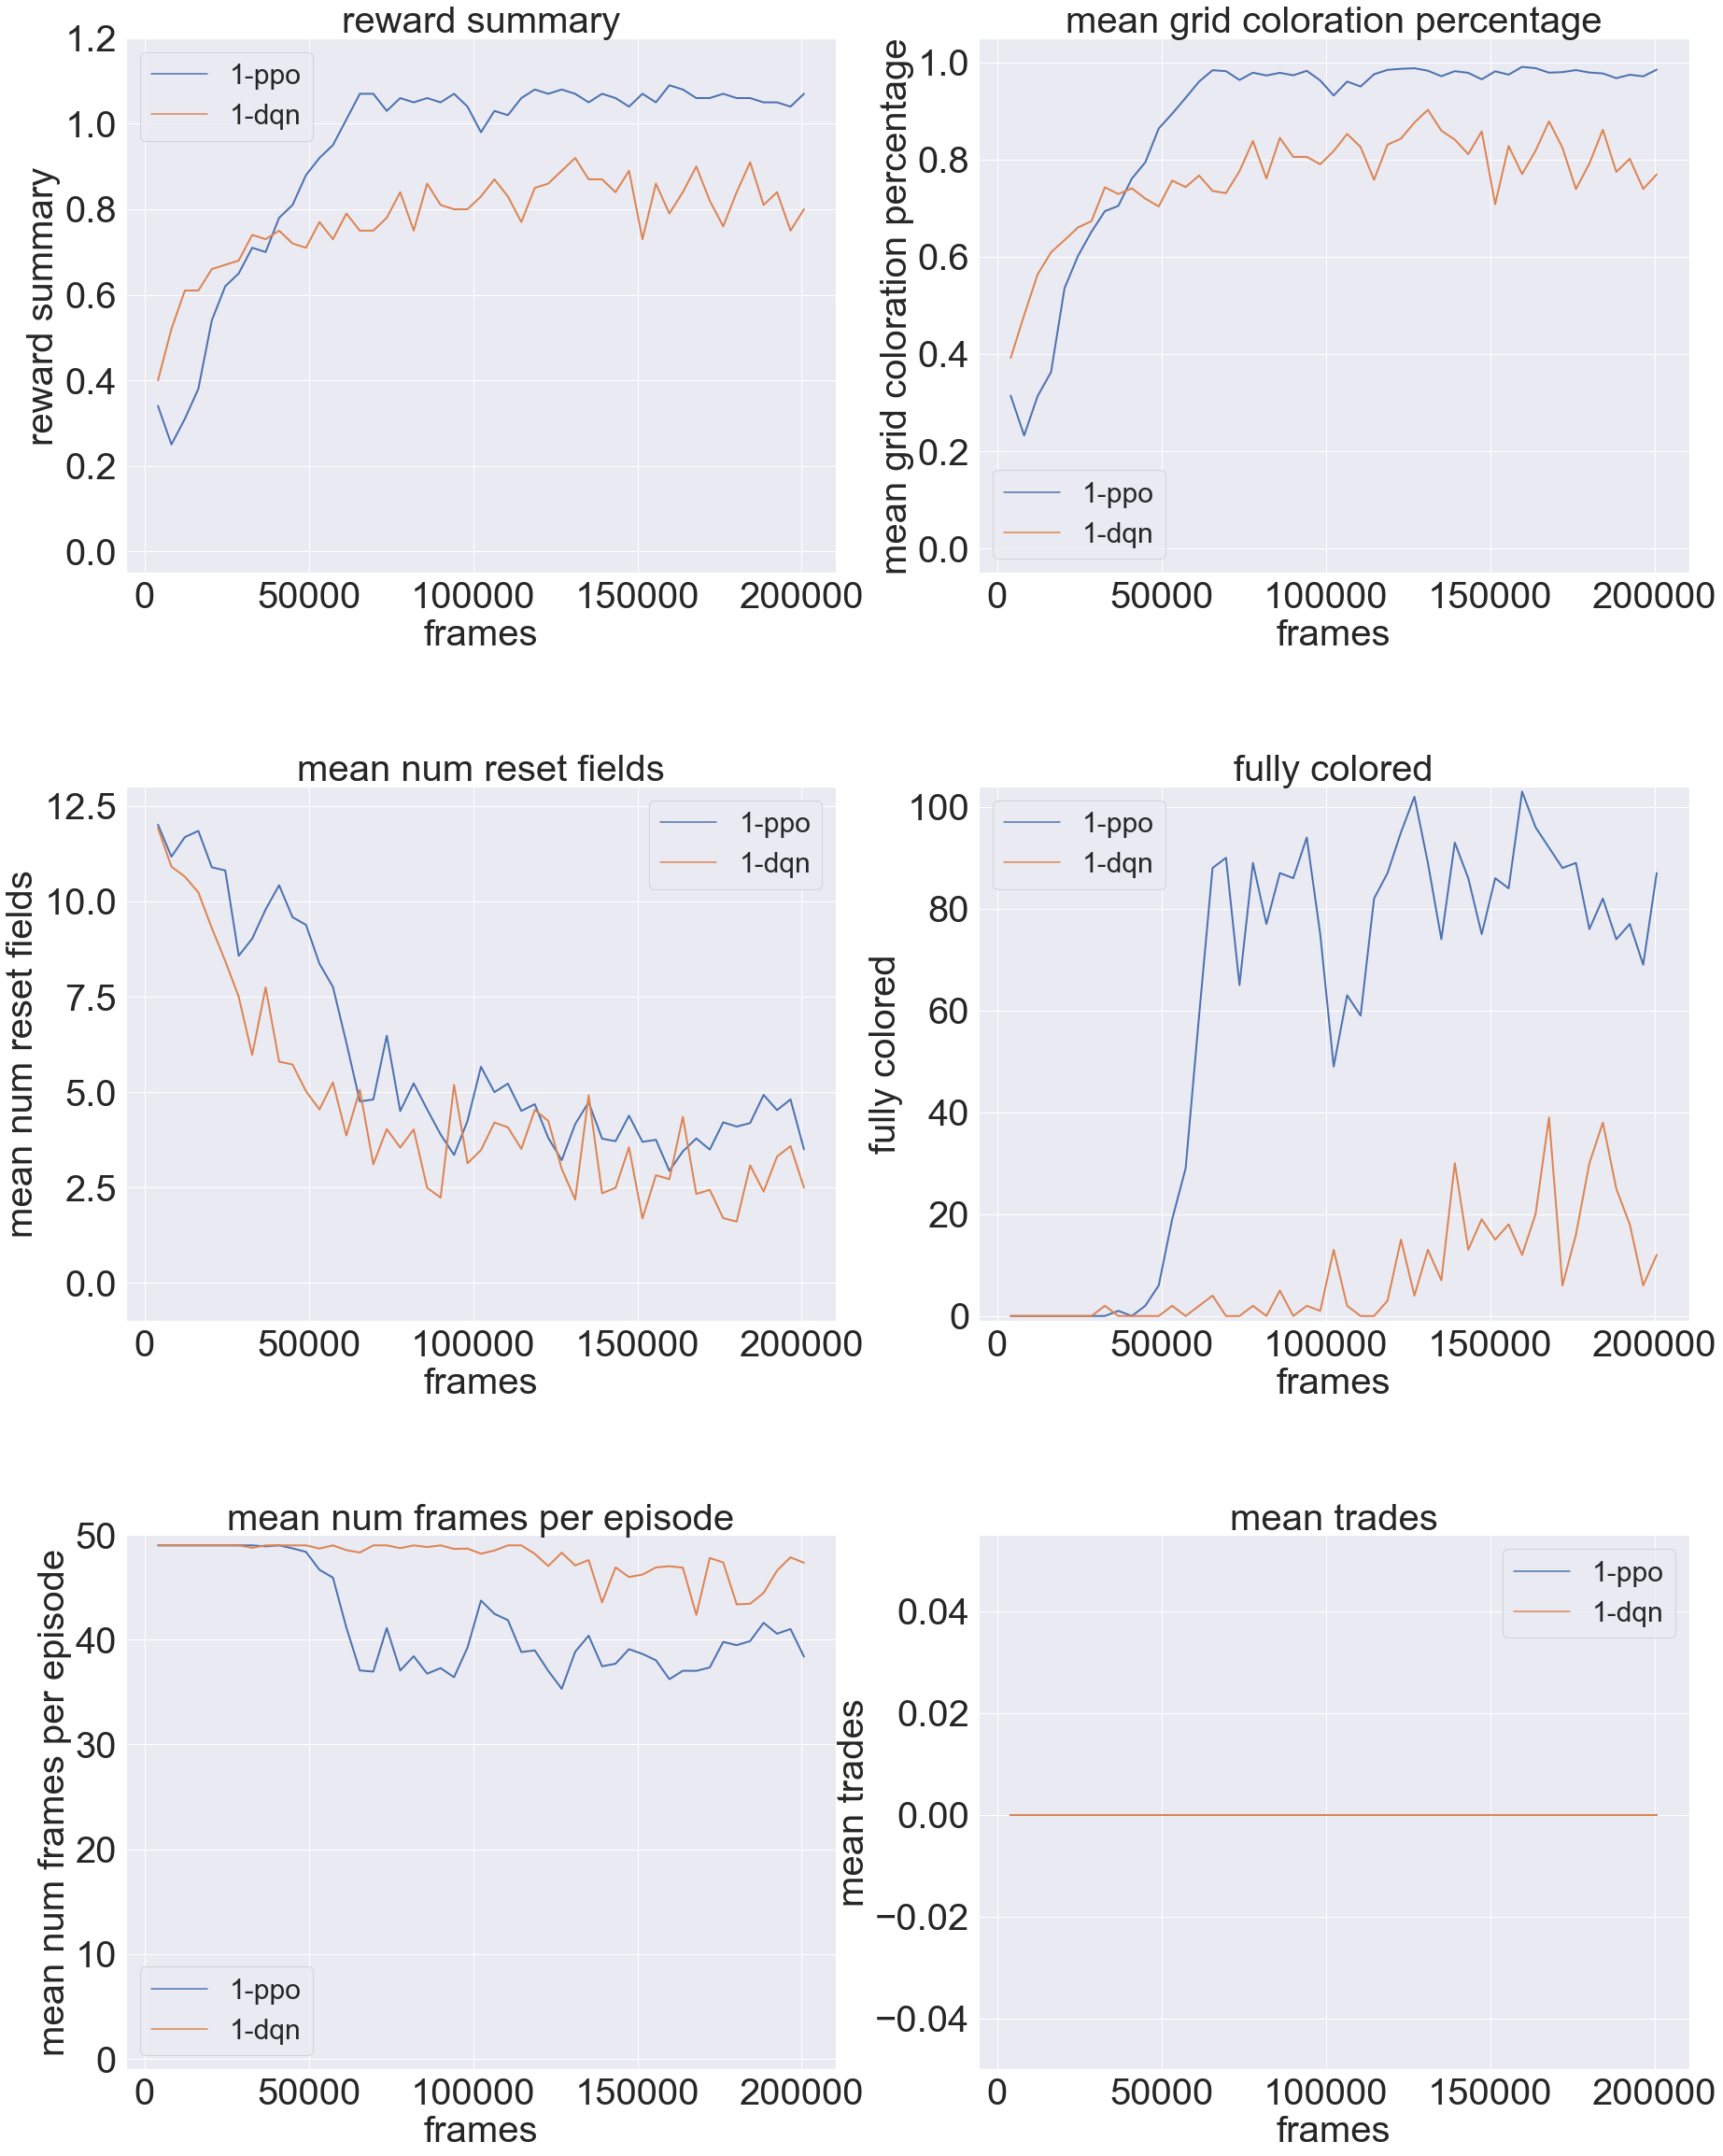
\includegraphics[width=1\textwidth]{AX-hard-1.png}\\
    \caption[PPO and DQN Training Details with One Agent in a 7x7 Environment]{Details of the training  in a 7x7 Environment with one agent using PPO and DQN}\label{fig:ax-hard-1}
\end{figure}
\vfill
\clearpage


\newpage
\vfill
\begin{figure}
    \centering
    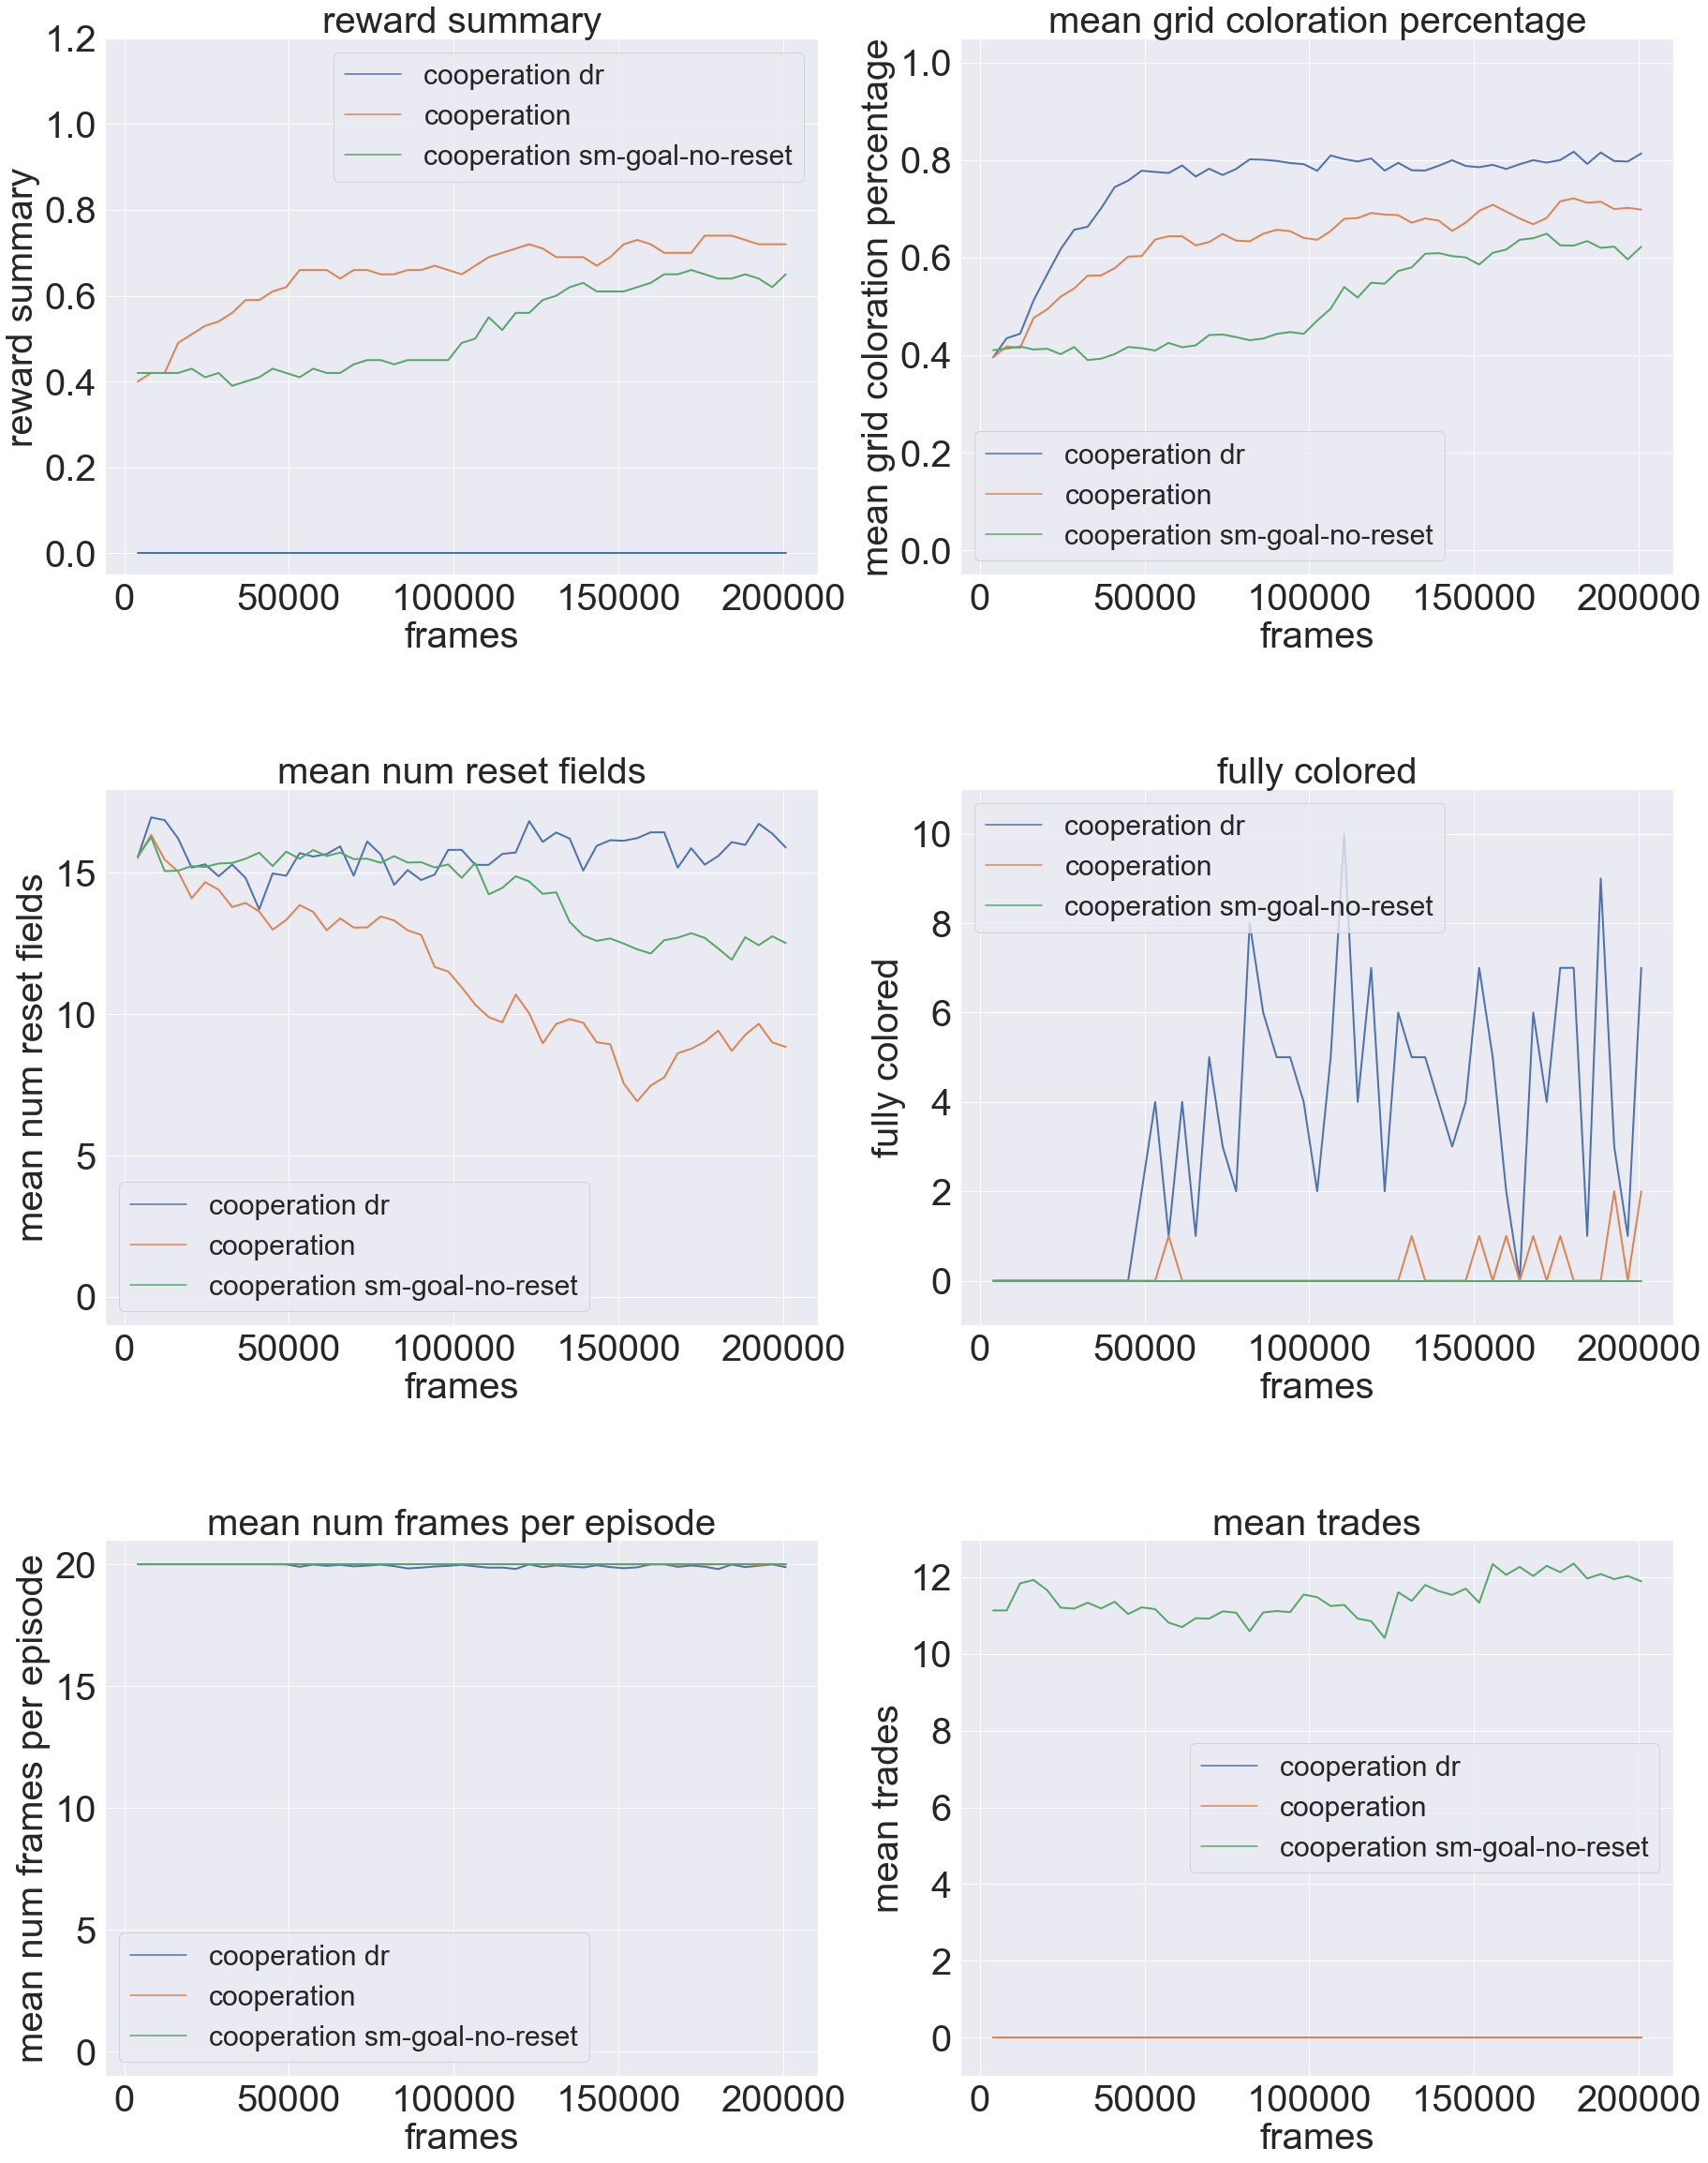
\includegraphics[width=1\textwidth]{AX-hard-3-ppo-coop.png}\\
    \caption[Training Details of Top PPO Cooperation Executions in a 7x7 Environment]{Top cooperation score details of three PPO agents in a 7x7 Environment}\label{fig:ax-hard-2-ppo-coop}
\end{figure}
\vfill
\clearpage


\newpage
\vfill
\begin{figure}
    \centering
    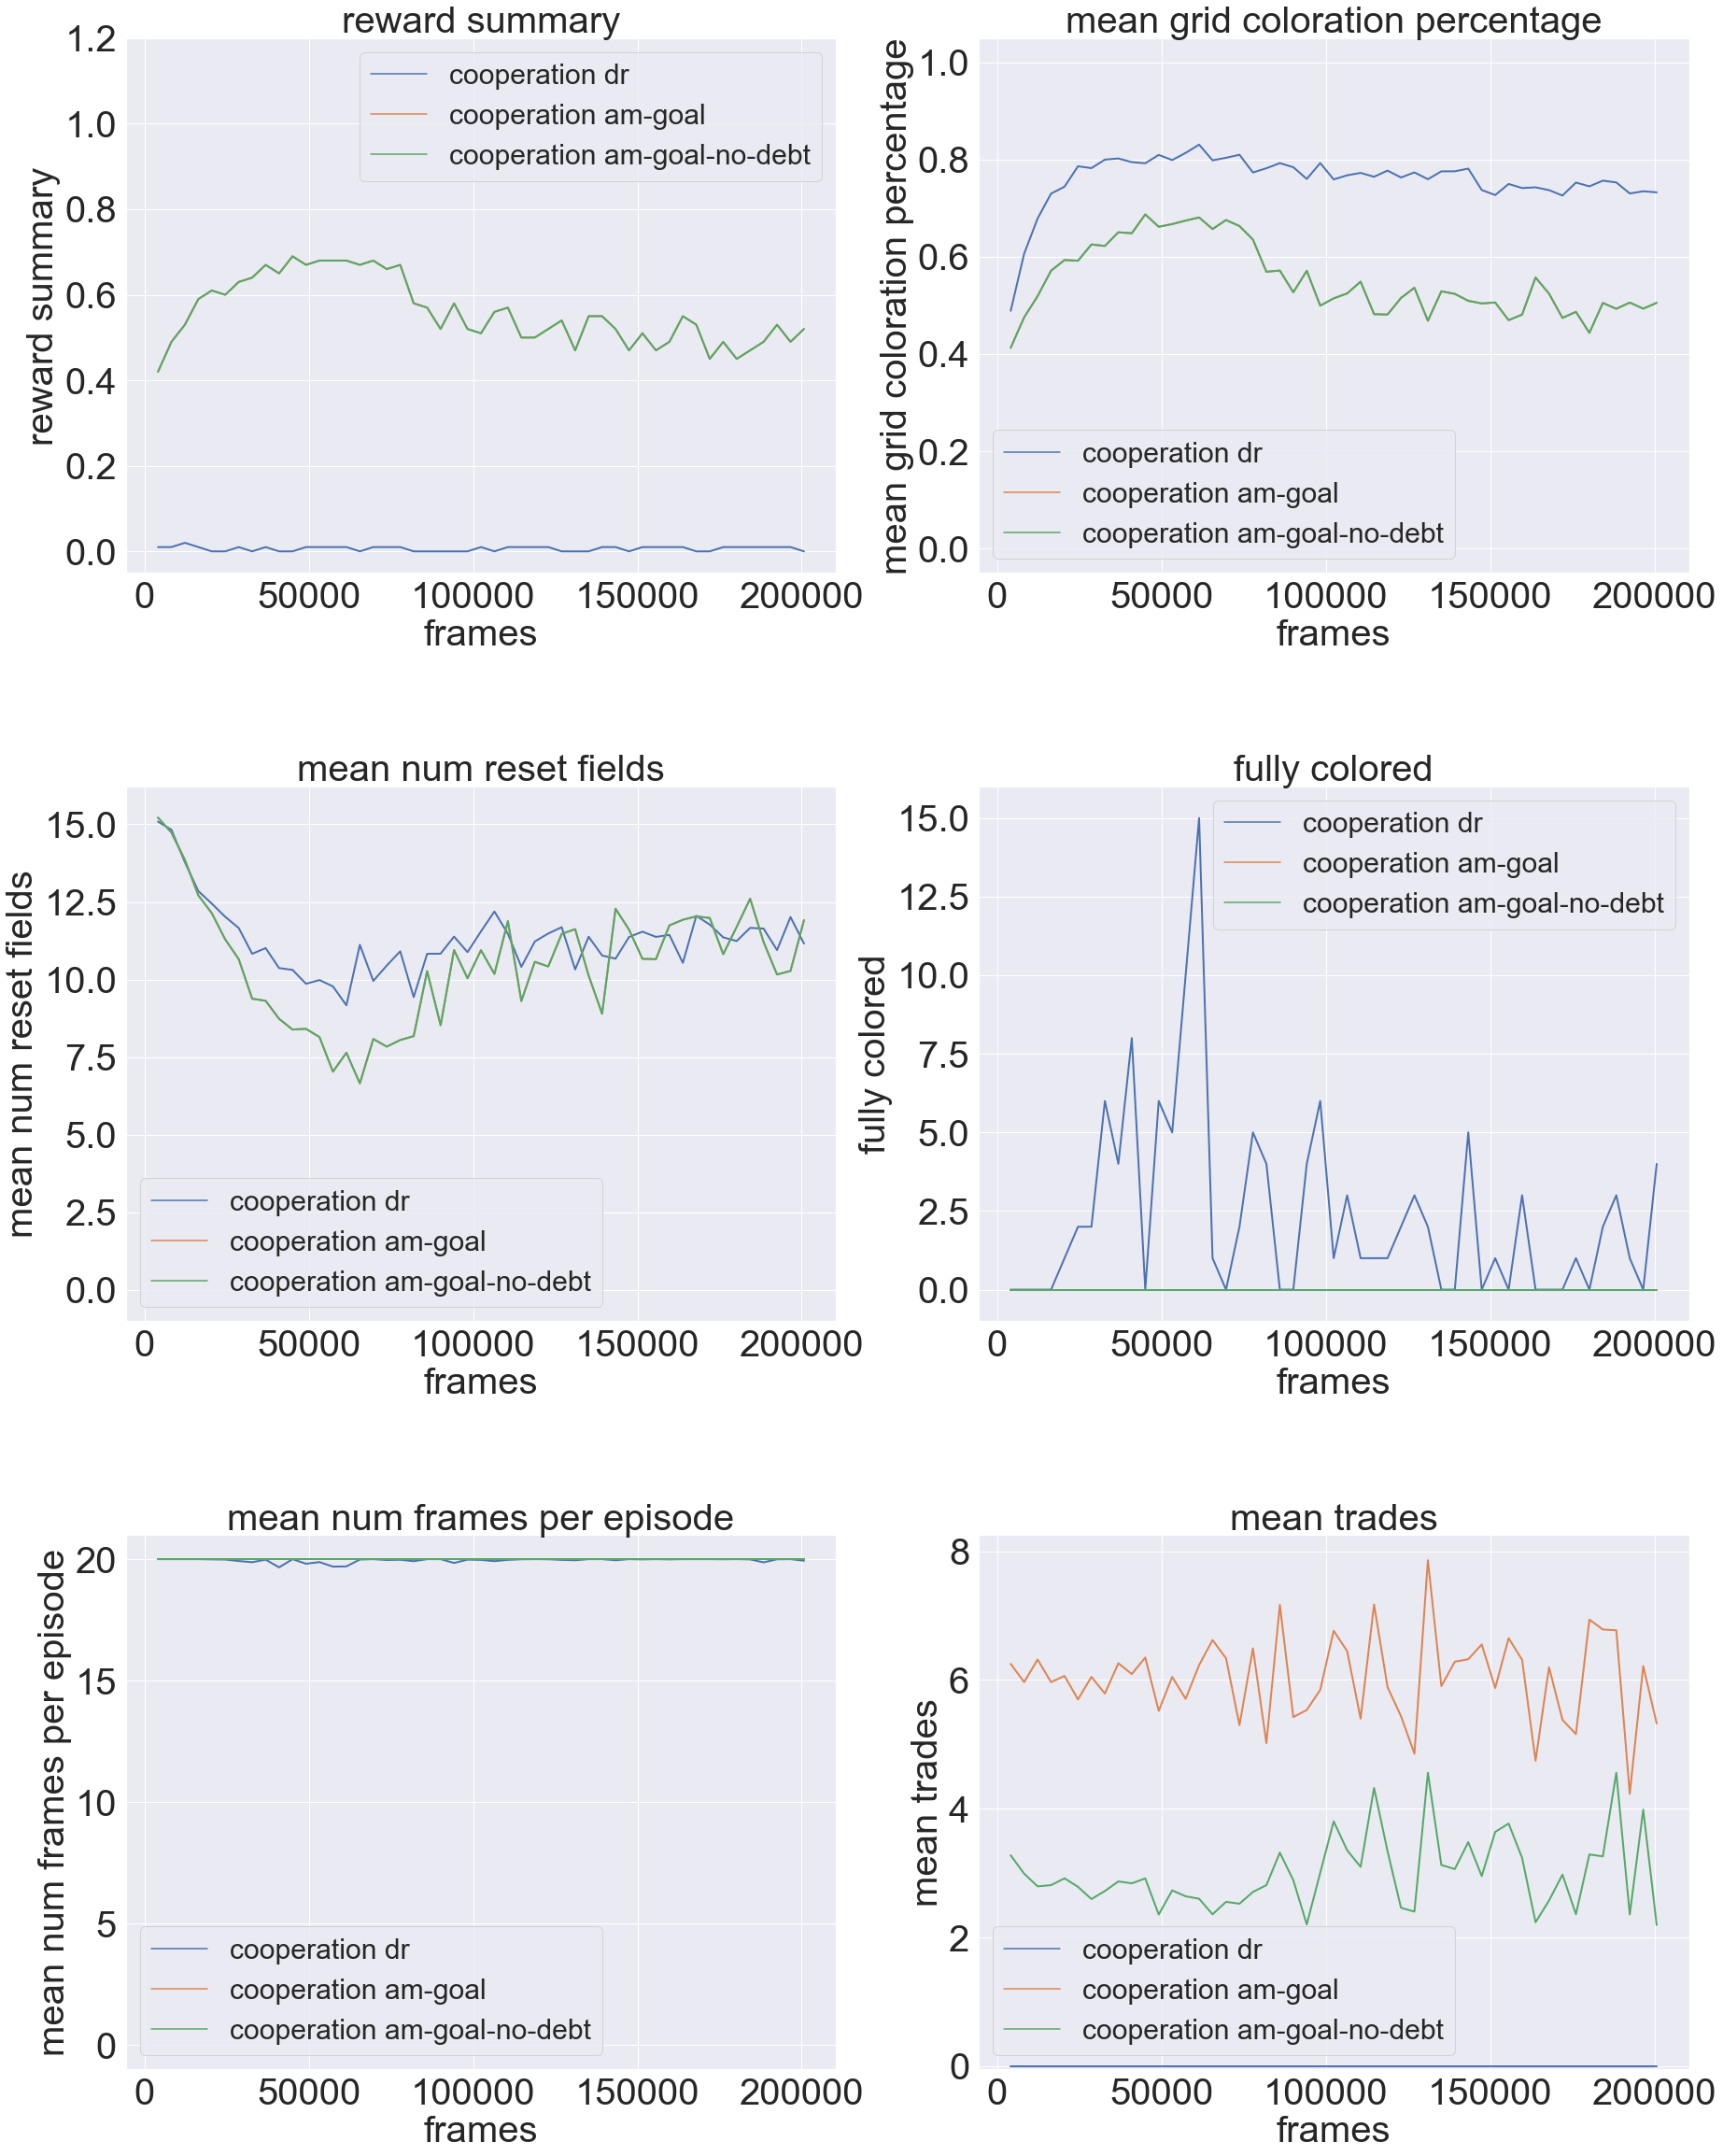
\includegraphics[width=1\textwidth]{AX-hard-3-dqn-coop.png}\\
    \caption[Training Details of Top DQN Cooperation Executions in a 7x7 Environment]{Top cooperation score details of three DQN agents in a 7x7 Environment}\label{fig:ax-hard-2-dqn-coop}
\end{figure}
\vfill
\clearpage


\newpage
\vfill
\begin{figure}
    \centering
    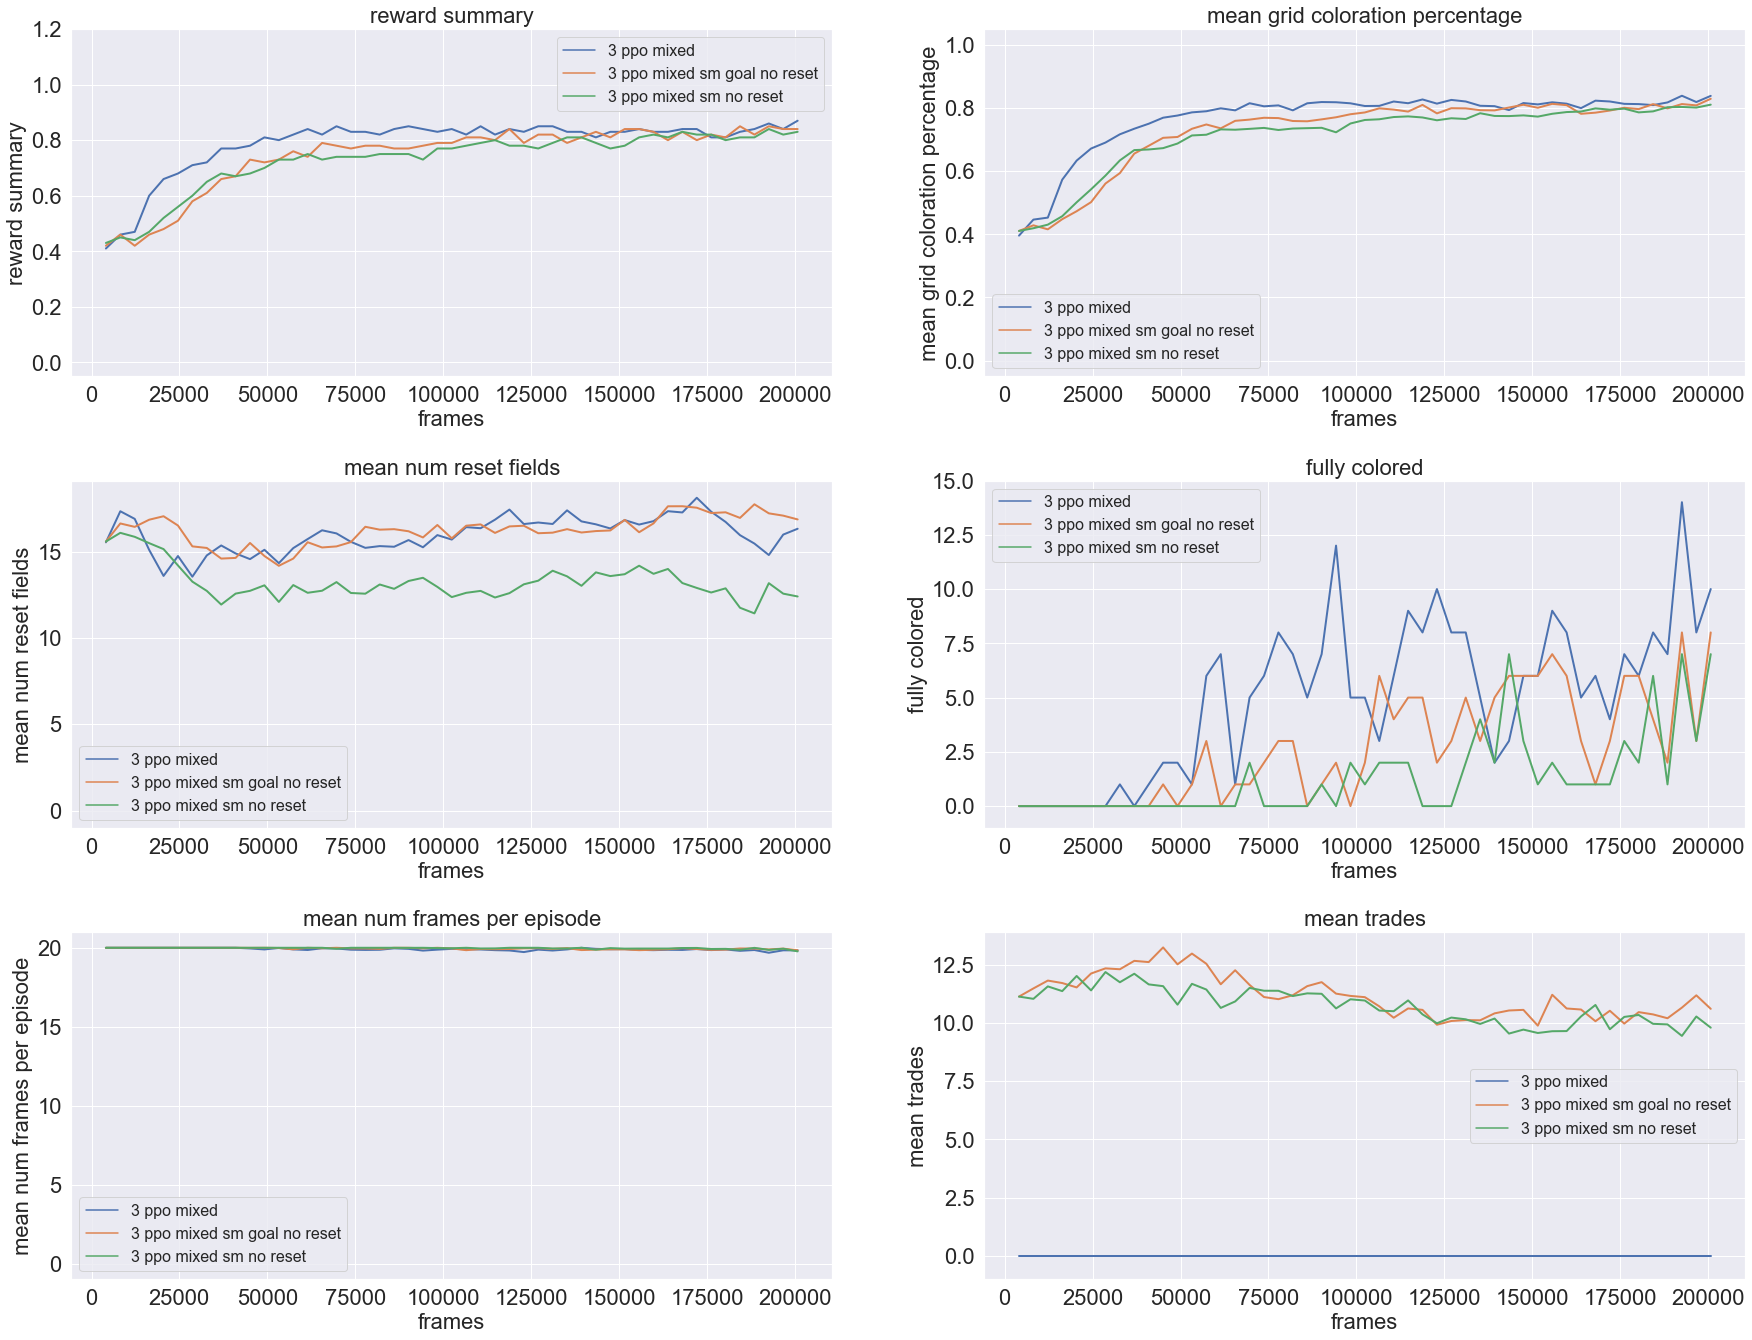
\includegraphics[width=1\textwidth]{AX-hard-3-ppo-mixed.png}\\
    \caption[Training Details of Top PPO Mixed-Motive Executions in a 7x7 Environment]{Top mixed-motive score details of three PPO agents in a 7x7 Environment}\label{fig:ax-hard-2-ppo-mixed}
\end{figure}
\vfill
\clearpage


\newpage
\vfill
\begin{figure}
    \centering
    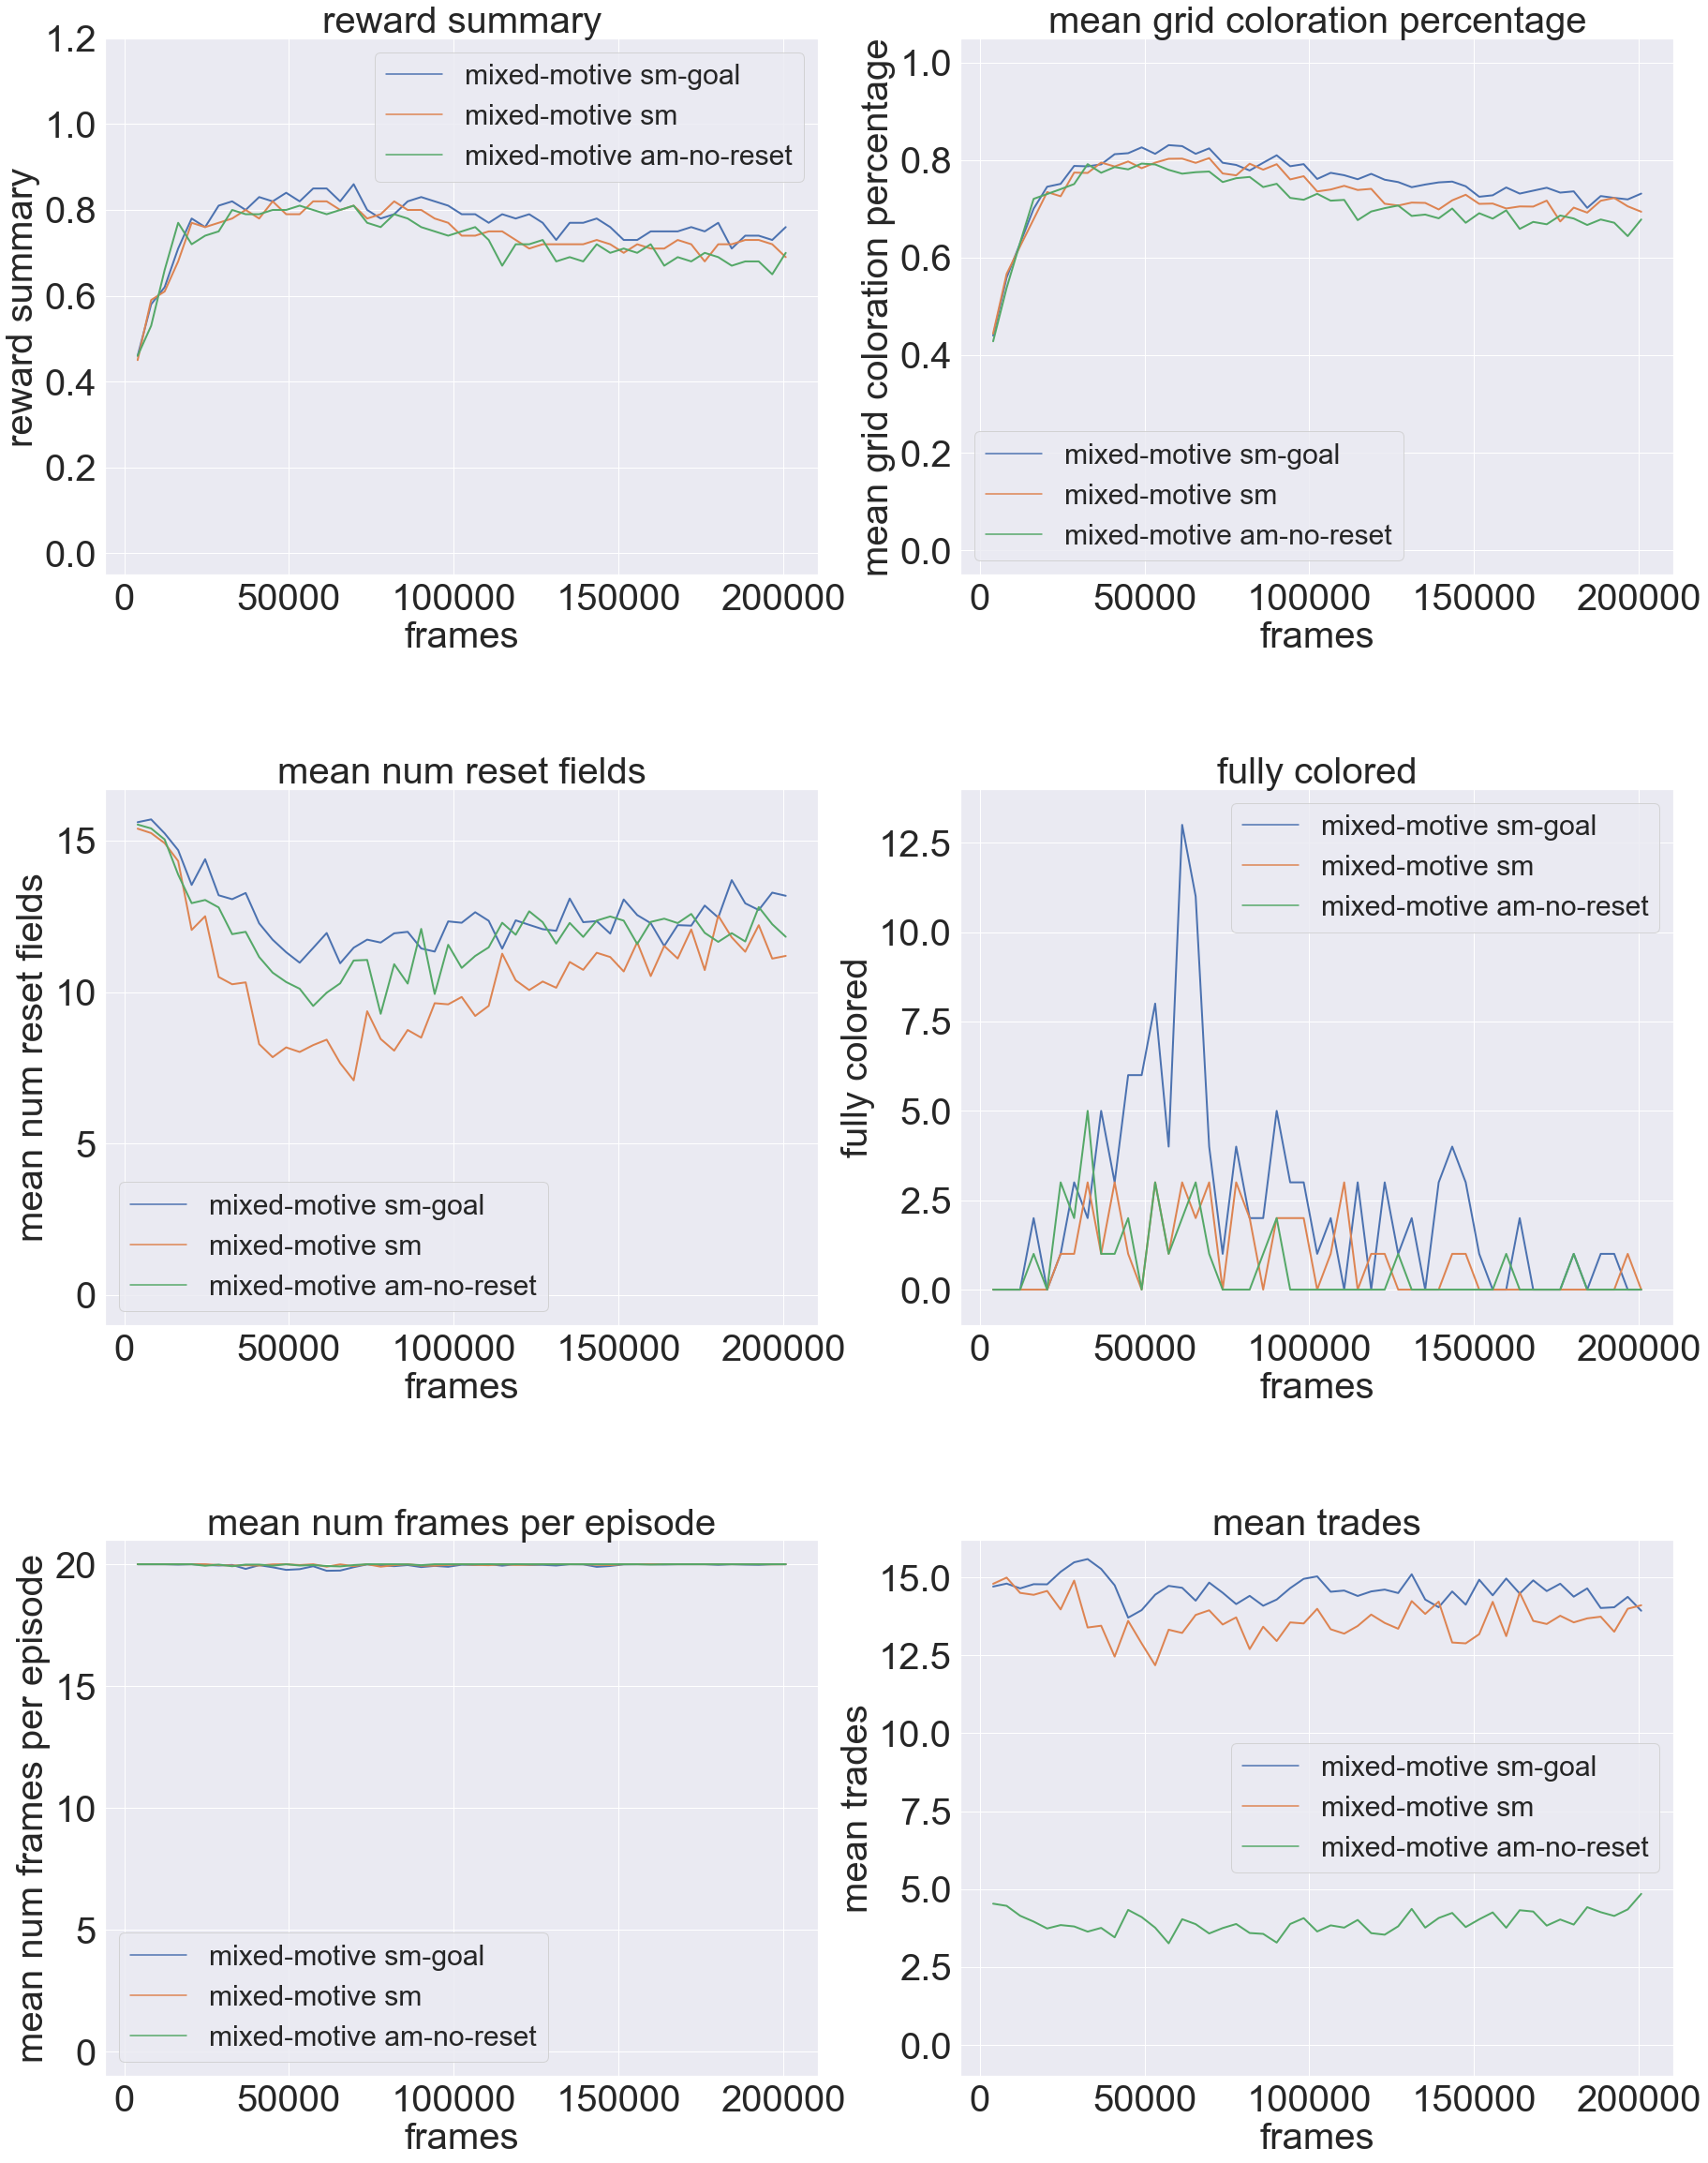
\includegraphics[width=1\textwidth]{AX-hard-3-dqn-mixed.png}\\
    \caption[Training Details of Top DQN Mixed-Motive Executions in a 7x7 Environment]{Top mixed-motive score details of three DQN agents in a 7x7 Environment}\label{fig:ax-hard-2-dqn-mixed}
\end{figure}
\vfill
\clearpage


\newpage
\vfill
\begin{figure}
    \centering
    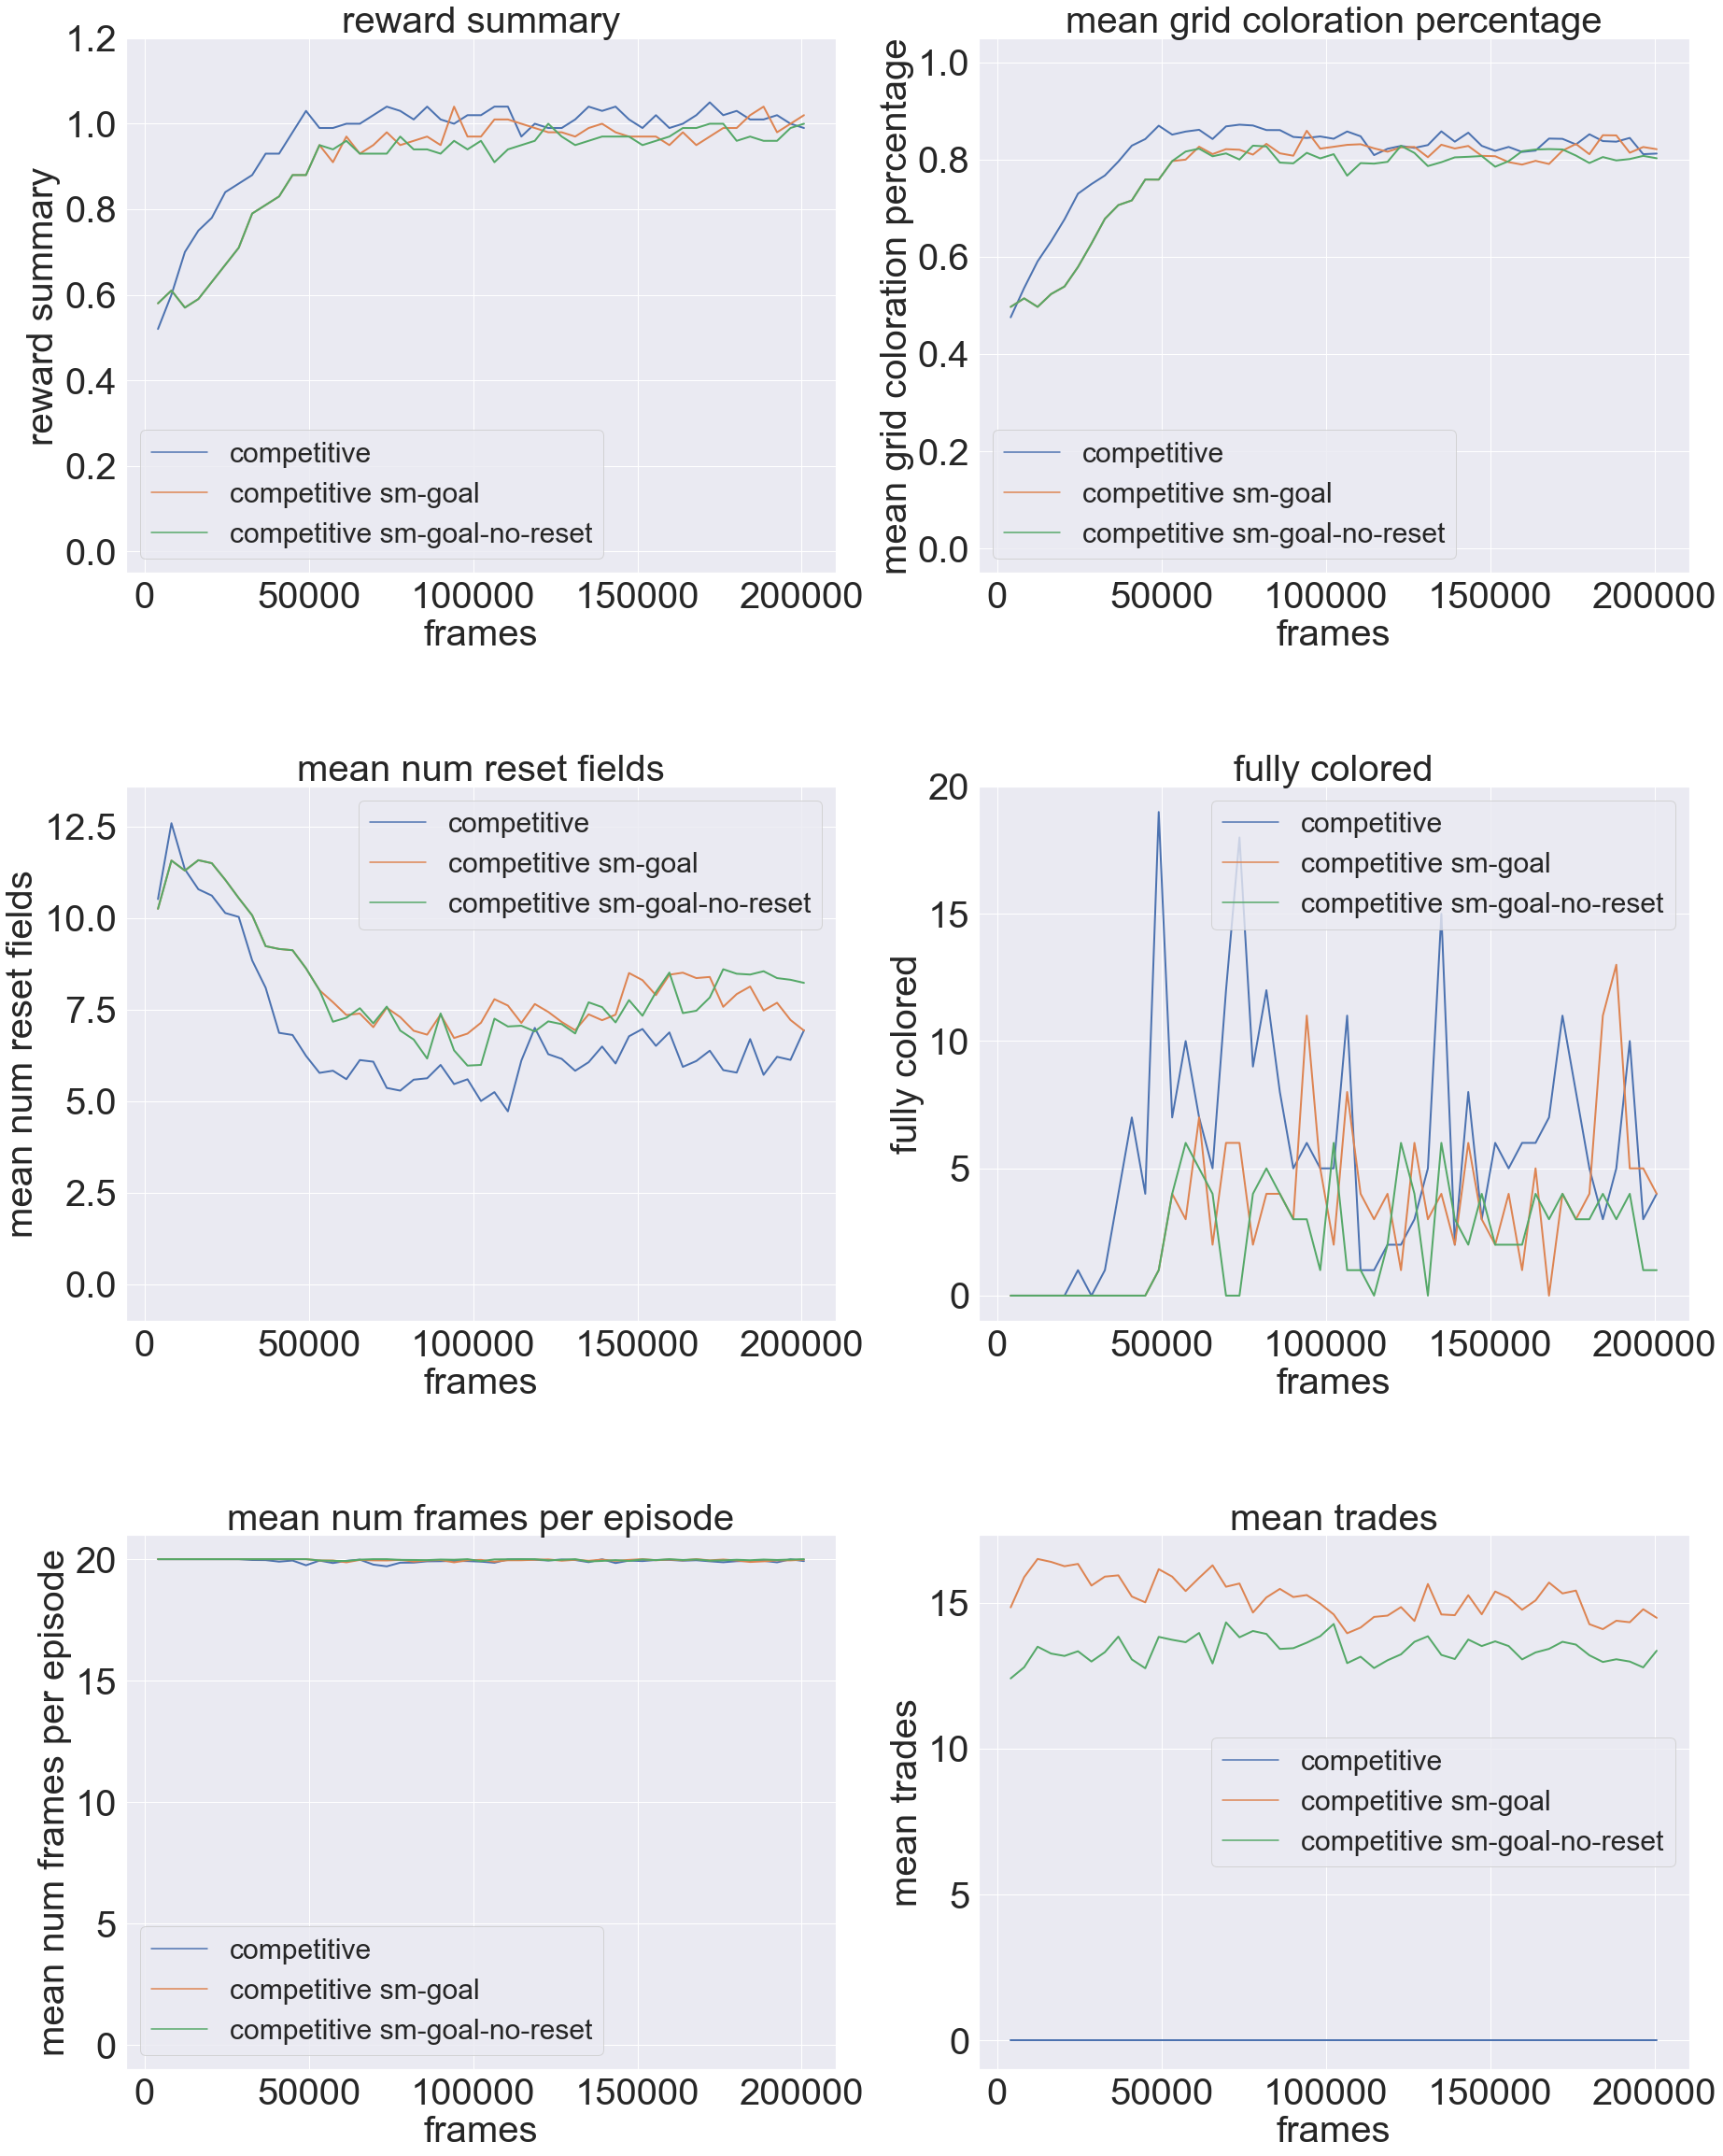
\includegraphics[width=1\textwidth]{AX-hard-3-ppo-comp.png}\\
    \caption[Training Details of Top PPO Competitive Executions in a 7x7 Environment]{Top competitive score details of three PPO agents in a 7x7 Environment}\label{fig:ax-hard-2-ppo-comp}
\end{figure}
\vfill
\clearpage


\newpage
\vfill
\begin{figure}
    \centering
    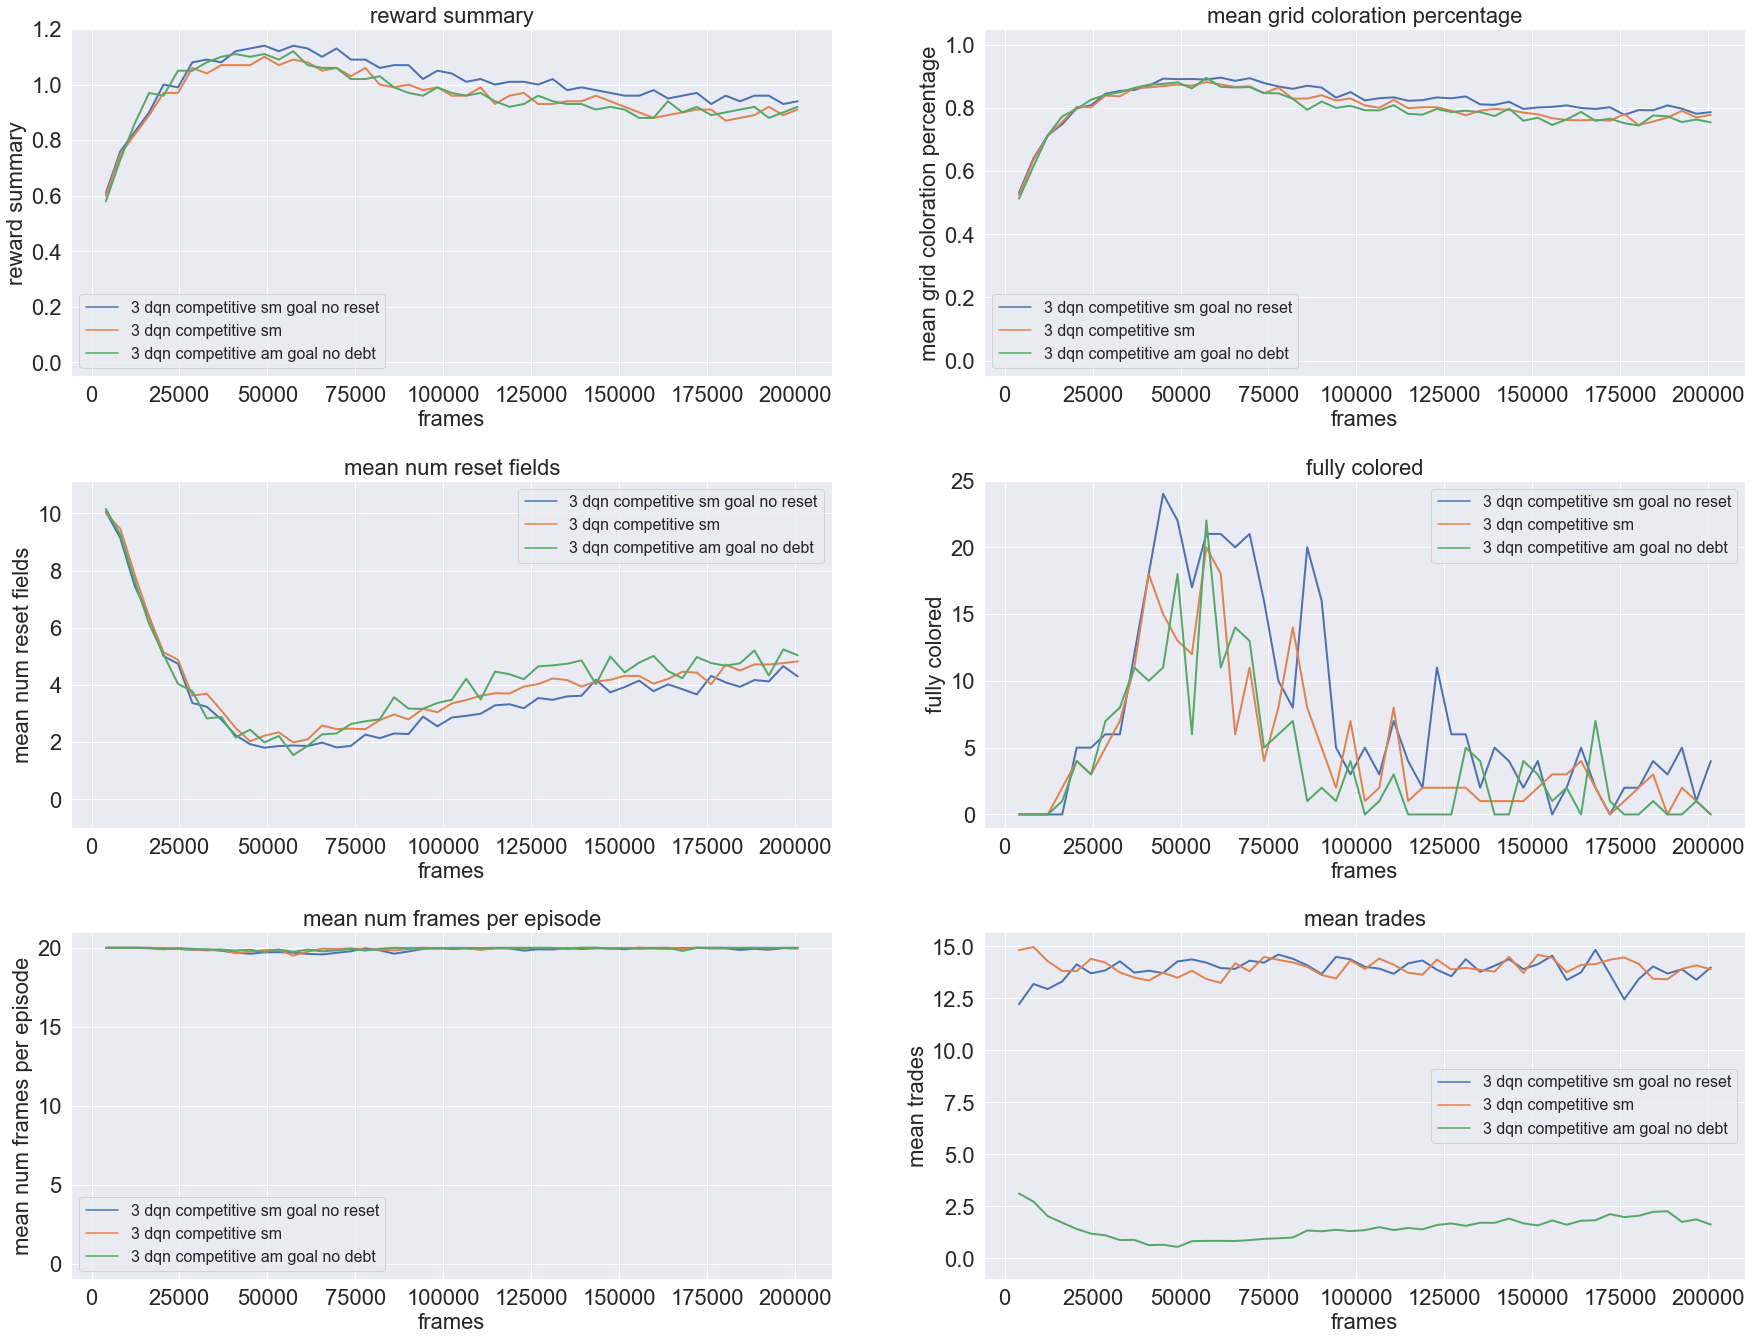
\includegraphics[width=1\textwidth]{AX-hard-3-dqn-comp.png}\\
    \caption[Training Details of Top DQN Competitive Executions in a 7x7 Environment]{Top competitive score details of three DQN agents in a 7x7 Environment}\label{fig:ax-hard-2-dqn-comp}
\end{figure}
\vfill
\clearpage


\subsection{Rooms Environment}
An example to run a training process in a nine by nine room divided environment is shown below.

\begin{lstlisting}[float=htp,language=bash, escapeinside={//@}{@//},xleftmargin=3ex,xrightmargin=1ex]
$ python -m scripts.train 
    --algo ppo 
    --agents 3 
    --model ppo-rooms
    --env FourRooms-Grid-v0 
    --grid-size 9 
    --max-steps 30 
    --frames-per-proc 256 
    --frames 200000 
\end{lstlisting}

\newpage
\vfill
\begin{figure}
    \centering
    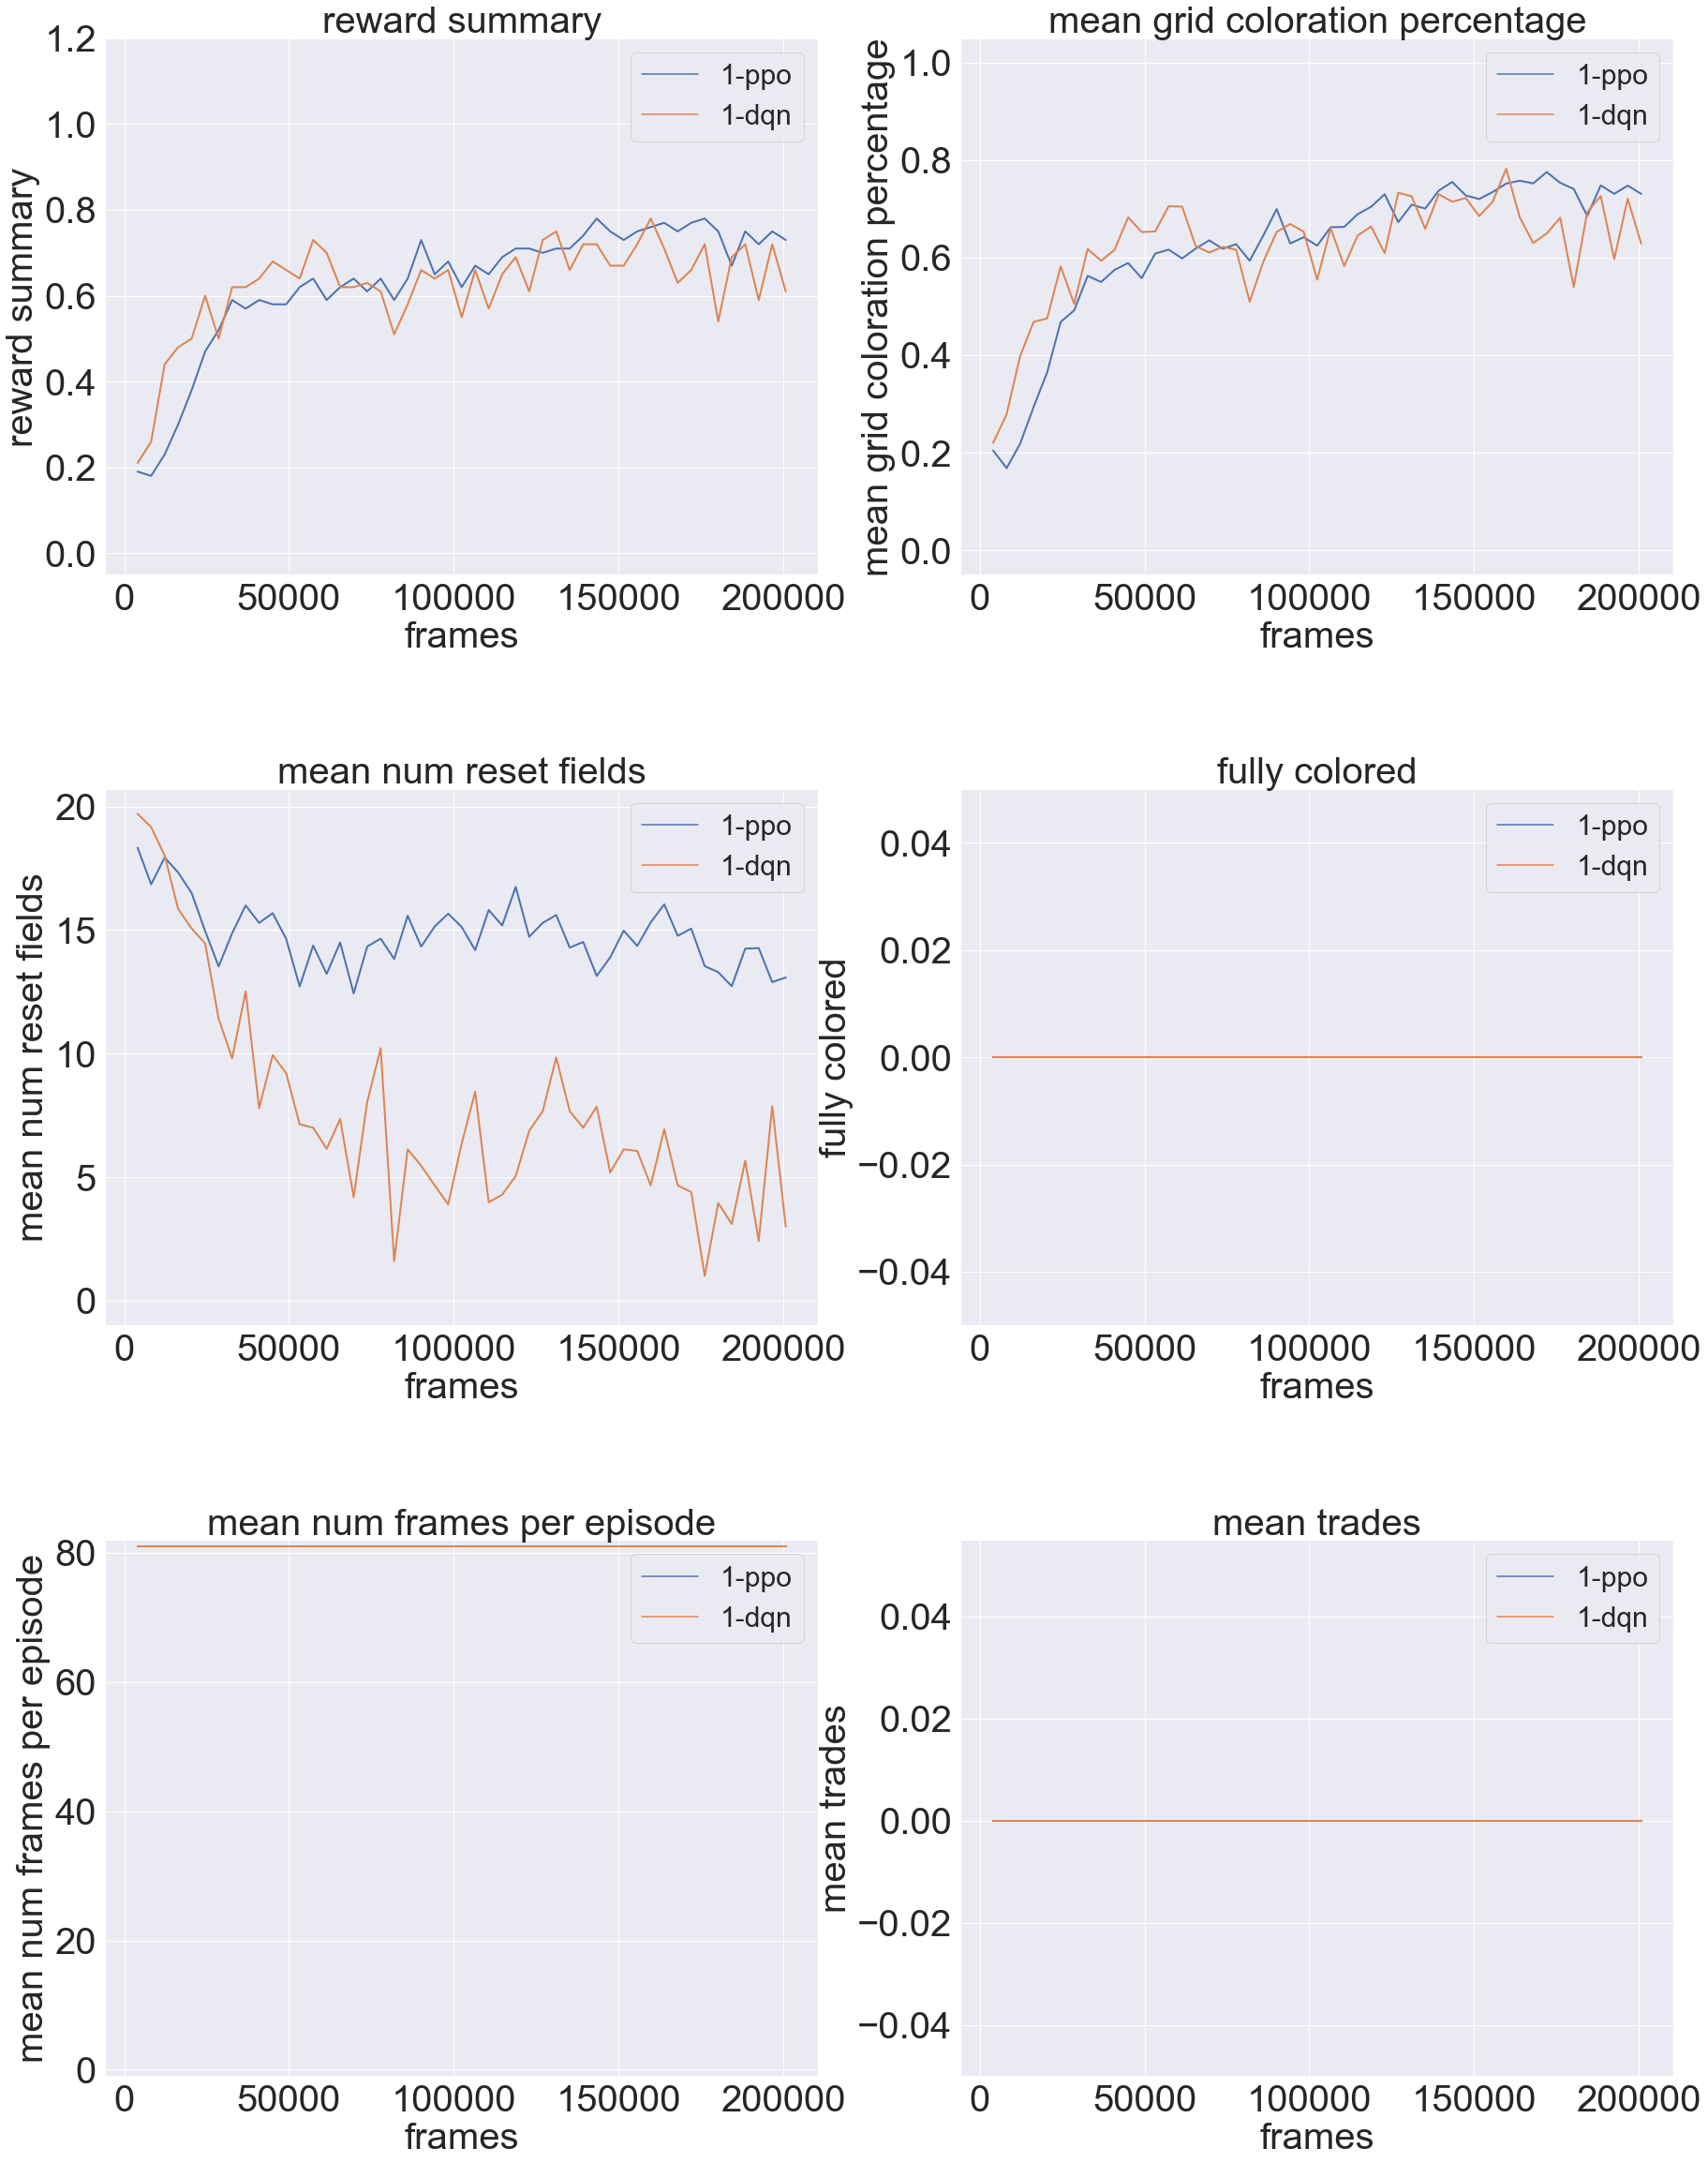
\includegraphics[width=1\textwidth]{AX-rooms-1.png}\\
    \caption[PPO and DQN Training Details with One Agent in a Rooms Environment]{Details of the training  in a 9x9 Rooms Environment with one agent using PPO and DQN}\label{fig:ax-rooms-1}
\end{figure}
\vfill
\clearpage


\newpage
\vfill
\begin{figure}
    \centering
    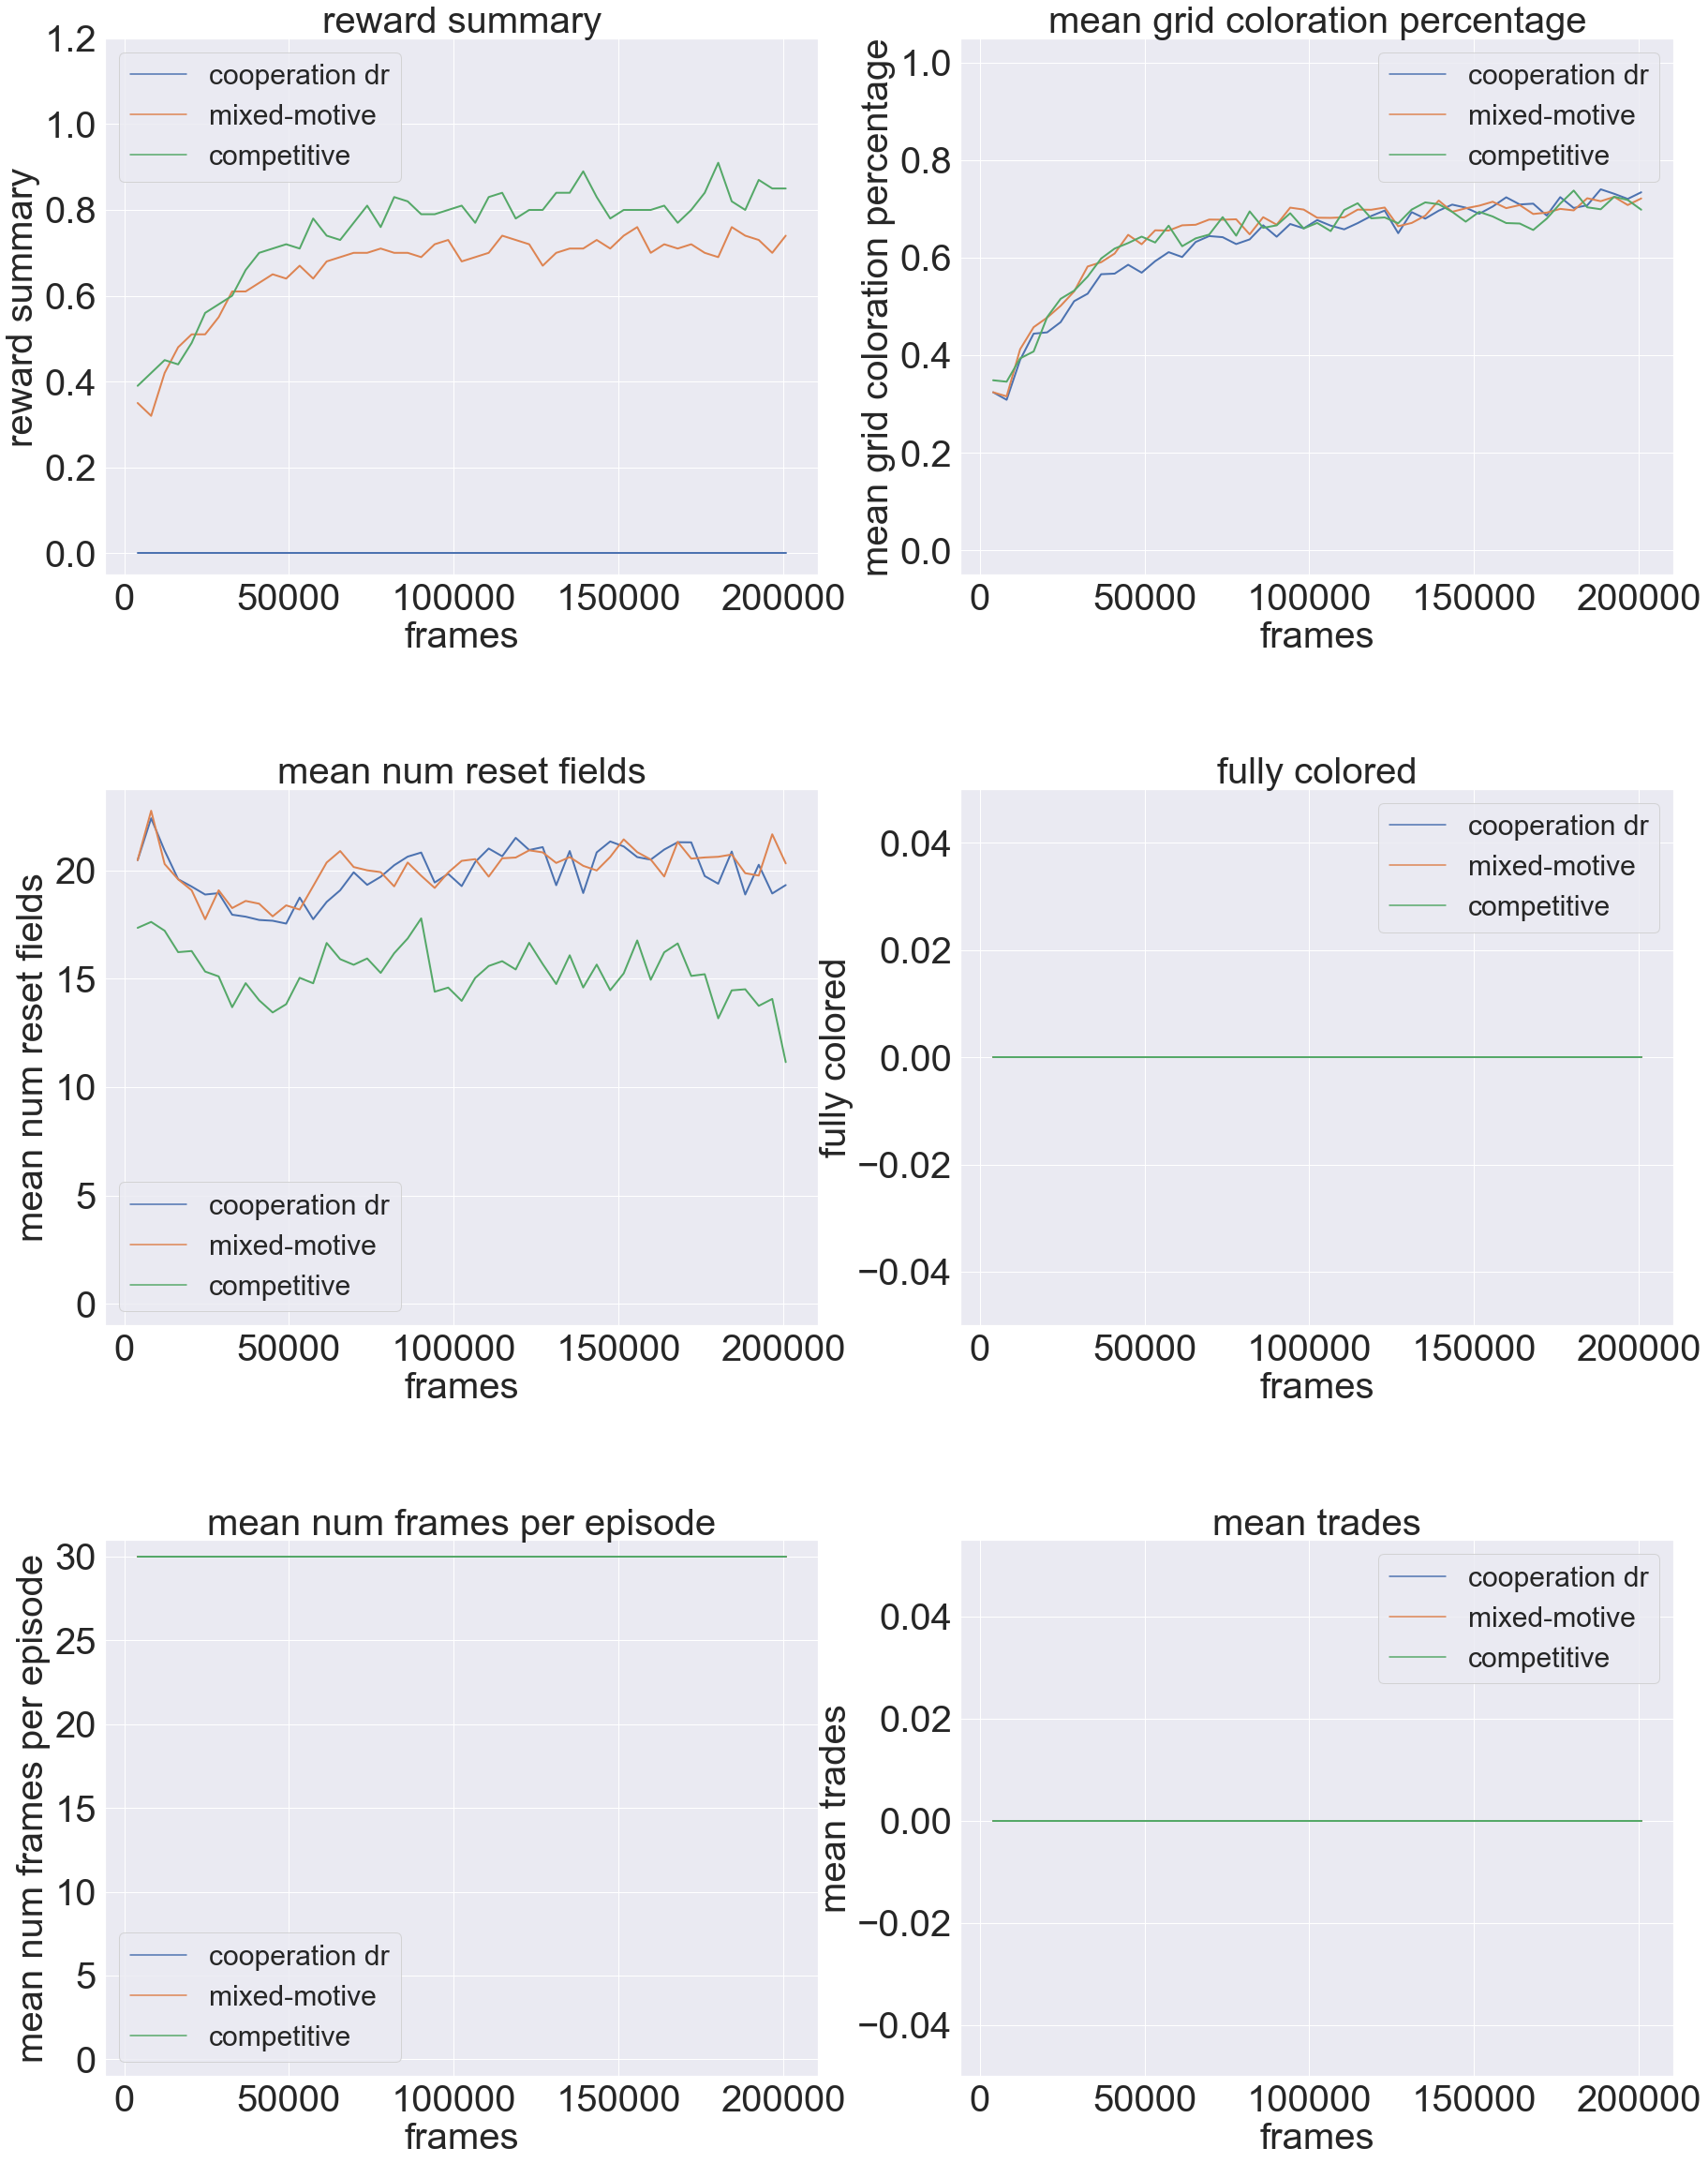
\includegraphics[width=1\textwidth]{AX-rooms-3-ppo.png}\\
    \caption[Training Details of Top PPO Competitive Executions in a Rooms Environment]{Top score details of three PPO agents in a 9x9 Rooms Environment}\label{fig:ax-rooms-3-ppo}
\end{figure}
\vfill
\clearpage


\newpage
\vfill
\begin{figure}
    \centering
    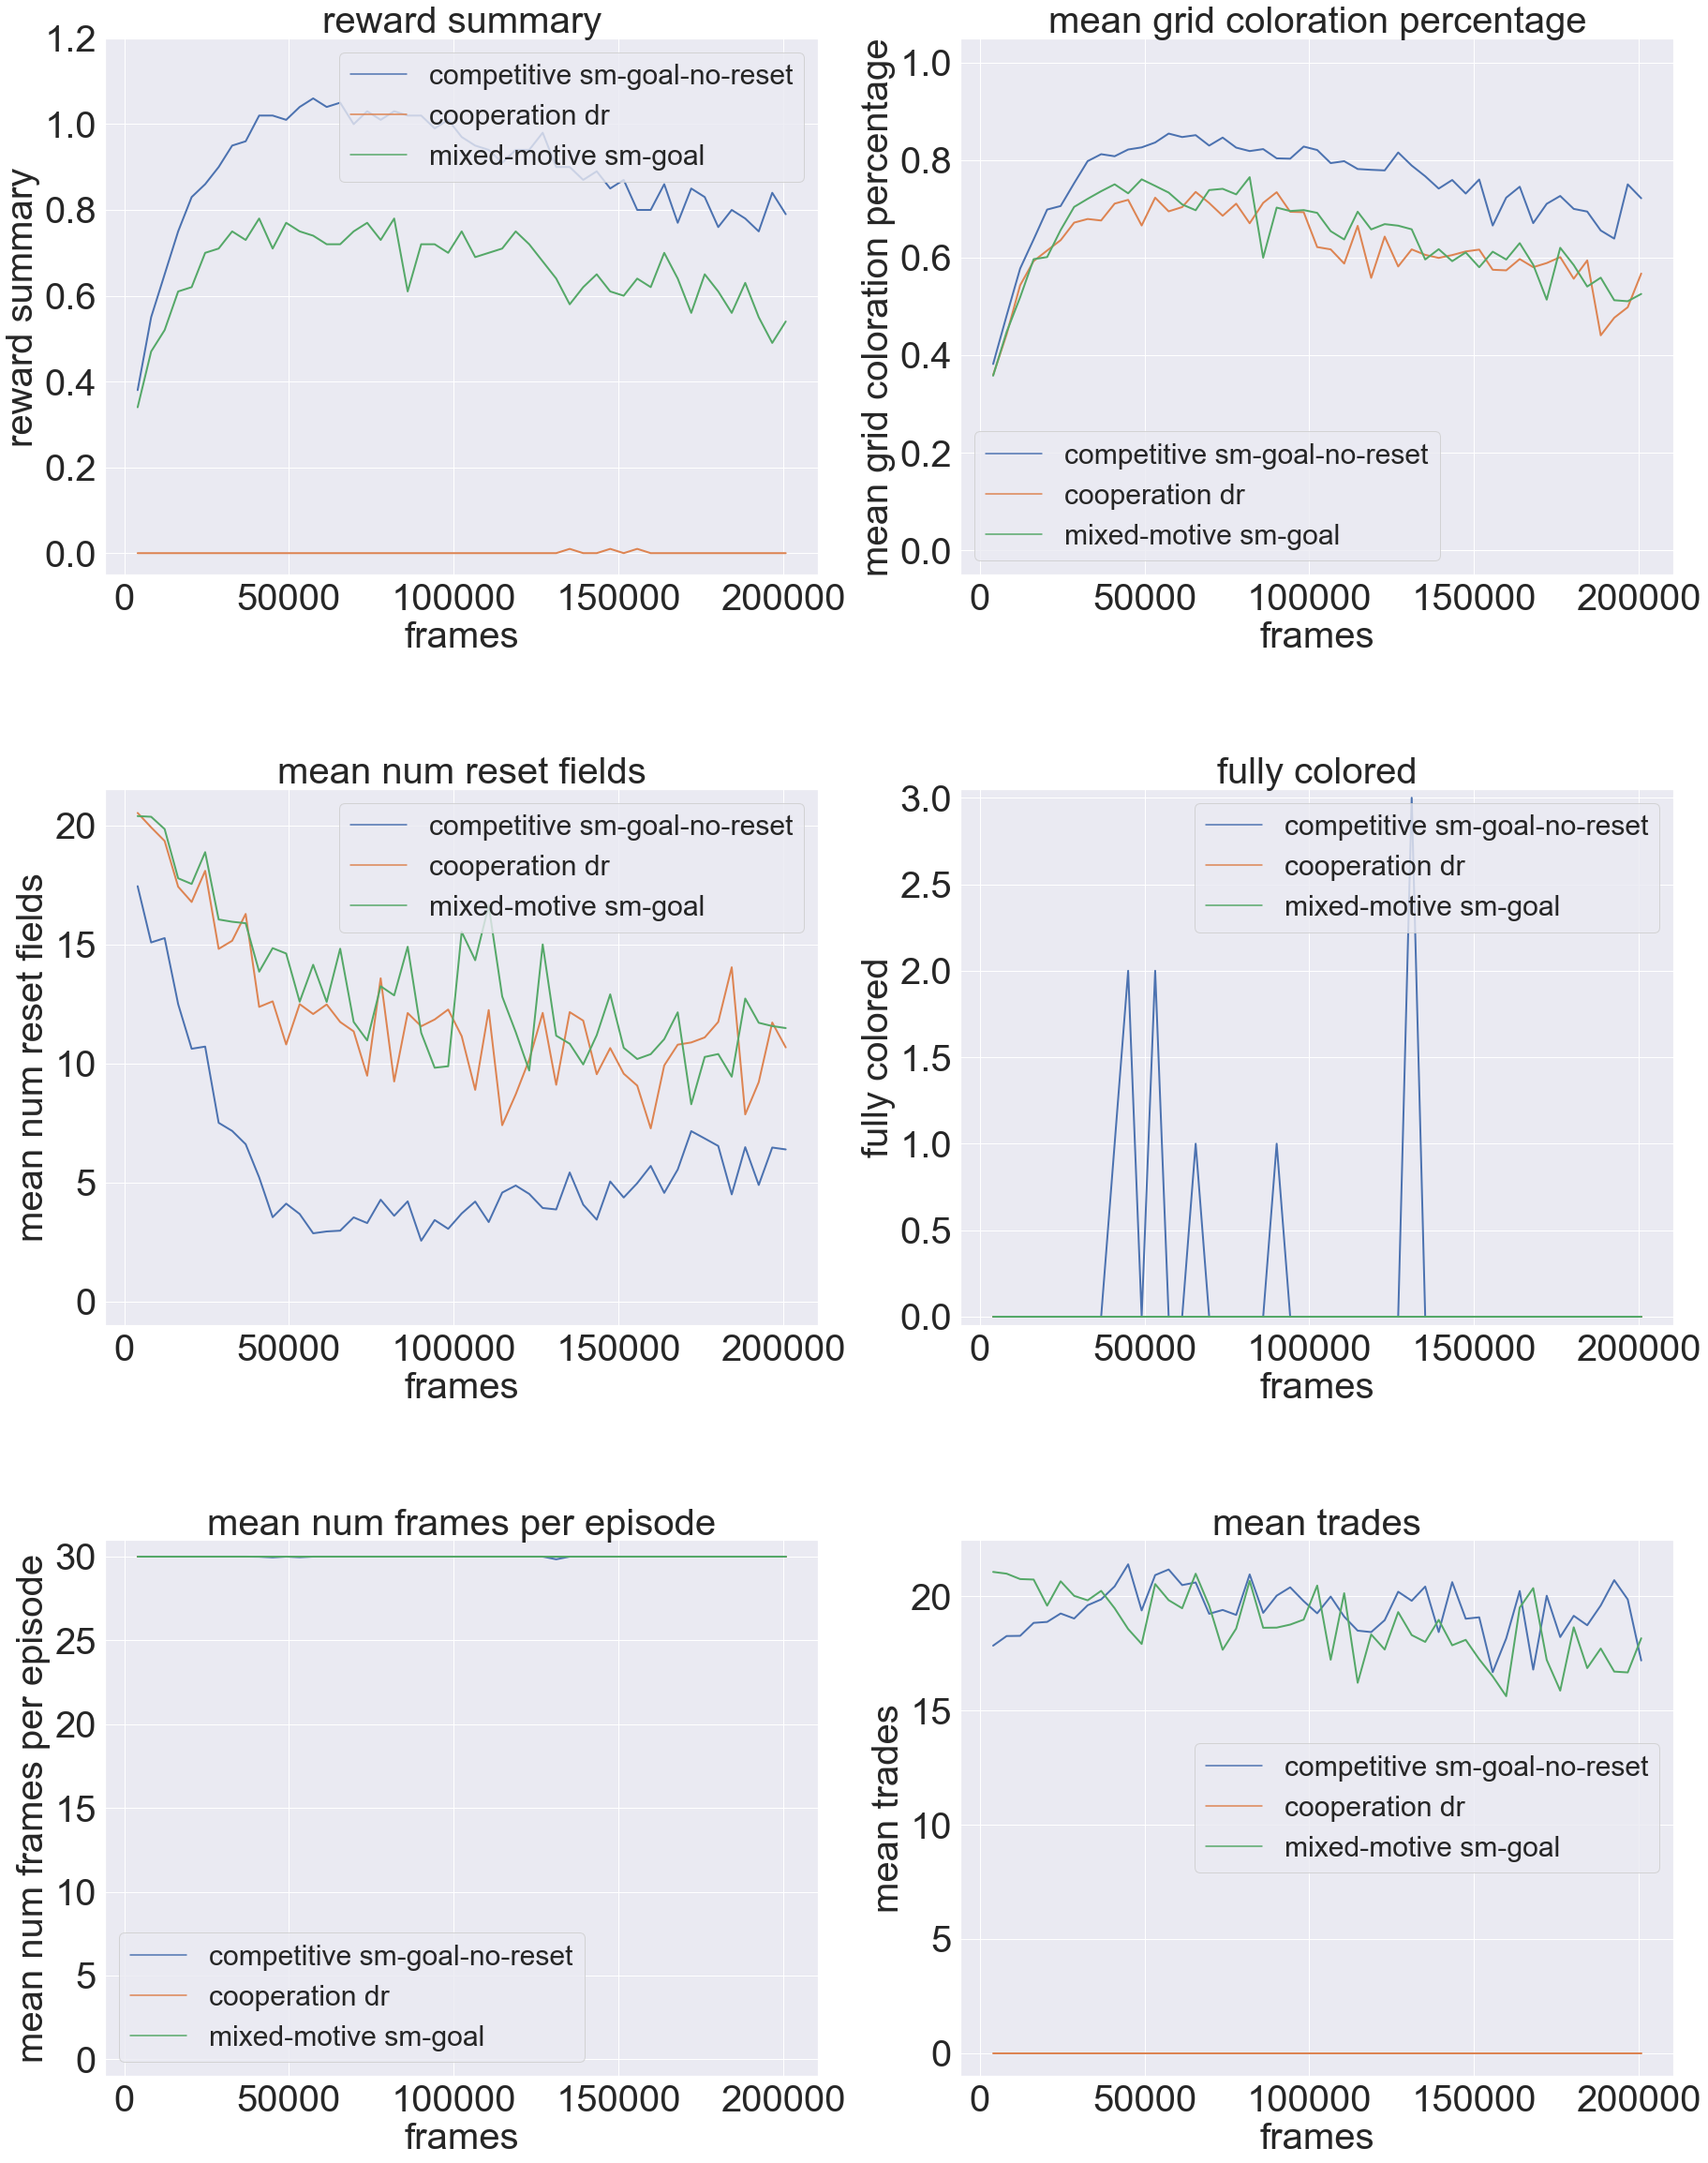
\includegraphics[width=1\textwidth]{AX-rooms-3-dqn.png}\\
    \caption[Training Details of Top DQN Competitive Executions in a Rooms Environment]{Top score details of three DQN agents in a 9x9 Rooms Environment}\label{fig:ax-rooms-3-dqn}
\end{figure}
\vfill
\clearpage
